% Relatório do Trabalho Prático (Etapa 2) — Locadora de Veículos.
% Formatação: modelo oficial da SBC (sbc-template.sty e sbc.bst, nesta pasta).
% Compilação:  pdflatex artigo && bibtex artigo && pdflatex artigo && pdflatex artigo
% Este arquivo é gerado por gerar_artigo.py a partir de conteudo.py.
\documentclass[12pt]{article}

\usepackage{sbc-template}
\usepackage{graphicx,url}
\usepackage[utf8]{inputenc}
\usepackage[T1]{fontenc}
\usepackage[brazilian]{babel}
\usepackage{array}
\usepackage{float}

\sloppy
\raggedbottom  % evita esticar títulos e parágrafos quando uma figura não cabe no fim da página

\title{Locadora de Veículos: integração entre frontend React, API ASP.NET Core e SQL Server}
\author{Caio Moraes da Silva\inst{1}}
\address{Pontifícia Universidade Católica de Minas Gerais — PUC Minas, Unidade Betim\\
  Disciplina: Tecnologias para Análise e Desenvolvimento de Sistemas
  \email{1556029@pucminas.edu.br}
}

\begin{document}

\maketitle

\begin{abstract}
  This paper presents the second stage of a vehicle rental system: a React and TypeScript frontend integrated, through an ASP.NET Core REST API, with a SQL Server database modeled with Entity Framework Core. It describes the data model, the architecture, 20 wireframes, CRUD for the five entities, filters and two SQL queries shown on screen (available vehicles and rentals by period). The solution uses the real API and database and was validated with 82 screen tests, 8 end-to-end tests and an accessibility scan.
  \textbf{Keywords:} vehicle rental; React; ASP.NET Core; SQL Server; REST API.
\end{abstract}

\begin{resumo}
  Este trabalho apresenta a segunda etapa de um sistema para locadora de veículos: um frontend em React e TypeScript integrado, por meio de uma API REST em ASP.NET Core, a um banco SQL Server modelado com Entity Framework Core. Descrevem-se a modelagem, a arquitetura, 20 wireframes, o CRUD das cinco entidades, os filtros e duas consultas SQL exibidas nas telas (veículos disponíveis e aluguéis por período). A solução usa a API e o banco reais e foi validada com 82 testes de telas, 8 testes ponta a ponta e verificação de acessibilidade.
  \textbf{Palavras-chave:} locadora de veículos; React; ASP.NET Core; SQL Server; API REST.
\end{resumo}

\section{Introdução}

Locadoras de veículos lidam com informações que mudam o tempo todo: quais carros estão livres, quem está com cada um, quando devem voltar e quanto deve ser cobrado. Quando esse controle é feito de forma manual, aparecem aluguéis conflitantes, devoluções esquecidas e valores incorretos. Um sistema com banco de dados e interface web reduz esses erros ao concentrar as regras em um só lugar.

Este trabalho corresponde à \textbf{Etapa 2} de um projeto em duas partes. Na Etapa 1 foram construídos o modelo de dados, as migrations e uma API REST em ASP.NET Core com Entity Framework Core e SQL Server, documentada e testada pelo Swagger. Na Etapa 2 foi desenvolvido o frontend que consome essa API, com wireframes, telas de CRUD para todas as entidades, filtros e visualizações baseados nas consultas do banco. O trabalho é individual, foi desenvolvido na disciplina Tecnologias para Análise e Desenvolvimento de Sistemas e o código está versionado em Git (repositório: \url{https://github.com/CaioM0RAES762/LocadoraVeiculos.git}).

O relatório segue o modelo de publicação de artigos da SBC \cite{sbc}. O restante do texto segue a ordem do desenvolvimento: problema e objetivos (Seção 2), modelagem (3), arquitetura e tecnologias (4), wireframes (5), telas (6), integração com a API (7), CRUD (8), filtros (9), as duas consultas de demonstração (10 e 11), testes (12), dificuldades (13) e conclusão (14).

\section{Descrição do problema e objetivos}

\subsection{Problema}

A locadora precisa cadastrar fabricantes, categorias, clientes e veículos, registrar aluguéis, acompanhar a situação de cada locação (em andamento, atrasada ou devolvida) e calcular o valor devido na devolução. Também precisa responder a perguntas do dia a dia: quais veículos estão disponíveis agora, quais aluguéis ocorreram em um período, qual o histórico de um cliente e quais clientes ainda não alugaram nenhum veículo.

\subsection{Objetivos}

\begin{itemize}
  \item Integrar frontend, API, back-end e banco de dados, reaproveitando todos os artefatos da Etapa 1 sem substituir o back-end;
  \item implementar cadastro, edição, exclusão e pesquisa para as cinco entidades, com filtros personalizados em pelo menos dois campos por entidade;
  \item expor no frontend as consultas SQL da Etapa 1 (JOINs) por meio das rotas já existentes;
  \item produzir wireframes de média/alta fidelidade e implementar as telas previstas;
  \item garantir qualidade com testes automatizados, inclusive contra o banco real, e com atenção à acessibilidade.
\end{itemize}

\section{Modelagem do banco de dados}

\subsection{Entidades e relacionamentos}

O modelo conceitual (Figura~\ref{fig:modelo}) foi definido na Etapa 1 e permanece inalterado na Etapa 2: a evolução do esquema não foi necessária, pois a disponibilidade de um veículo e a situação de um aluguel são derivadas das datas e calculadas nas consultas, em vez de armazenadas.

\begin{figure}[H]
  \centering
  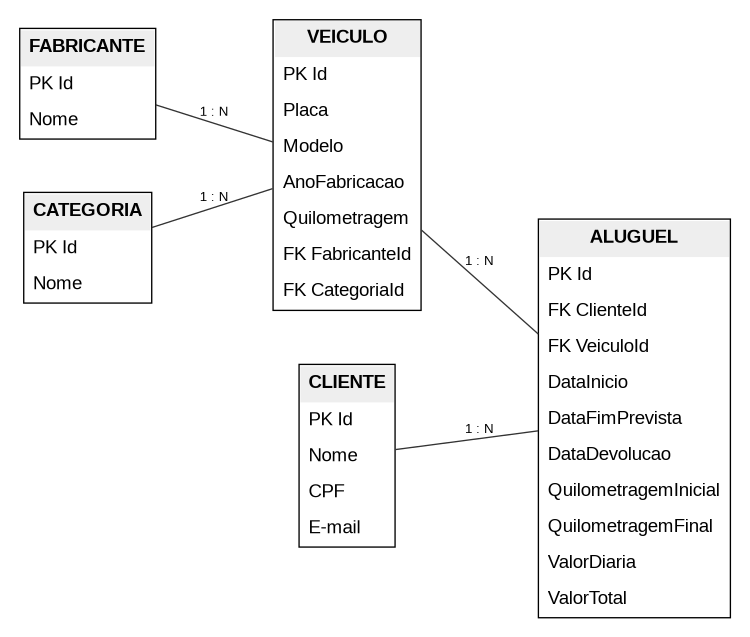
\includegraphics[width=11.0cm]{imagens/modelo-conceitual.png}
  \caption{Modelo conceitual do banco de dados (Etapa 1): cinco entidades e quatro relacionamentos 1:N.}
  \label{fig:modelo}
\end{figure}

\begin{table}[H]
  \centering
  \caption{Entidades e principais atributos.}
  \label{tab:entidades}
  \small
  \begin{tabular}{|>{\raggedright\arraybackslash}p{2.27cm}|>{\raggedright\arraybackslash}p{7.34cm}|>{\raggedright\arraybackslash}p{3.84cm}|}
  \hline
  \textbf{Entidade} & \textbf{Atributos} & \textbf{Relacionamentos} \\ \hline
  Fabricante & Id, Nome (único, até 100) & 1:N com Veículo \\ \hline
  Categoria & Id, Nome (único, até 80) & 1:N com Veículo \\ \hline
  Cliente & Id, Nome, CPF (11 dígitos, único), E-mail (único) & 1:N com Aluguel \\ \hline
  Veículo & Id, Placa (única), Modelo, AnoFabricacao, Quilometragem, FabricanteId, CategoriaId & N:1 com Fabricante e Categoria; 1:N com Aluguel \\ \hline
  Aluguel & Id, ClienteId, VeiculoId, DataInicio, DataFimPrevista, DataDevolucao, QuilometragemInicial, QuilometragemFinal, ValorDiaria, ValorTotal & N:1 com Cliente e Veículo \\ \hline
  \end{tabular}
\end{table}

\subsection{Regras de integridade}

O banco protege os dados com chaves estrangeiras \texttt{ON DELETE RESTRICT}, índices únicos (nome do fabricante e da categoria, CPF, e-mail e placa) e restrições \texttt{CHECK}: ano de fabricação maior ou igual a 1900, quilometragens não negativas, fim previsto posterior ao início, quilometragem final maior ou igual à inicial, diária positiva e total não negativo. A API repete essas validações e devolve mensagens claras: erros de formato retornam \texttt{400}, registros inexistentes \texttt{404} e violações de unicidade ou vínculo \texttt{409}. Um aluguel em aberto (sem data de devolução) impede um segundo aluguel em aberto do mesmo veículo.

\section{Arquitetura e tecnologias}

A aplicação segue uma arquitetura em quatro blocos (Figura~\ref{fig:arquitetura}). O navegador executa uma aplicação de página única (SPA) em React; em desenvolvimento, o servidor do Vite encaminha as chamadas a \texttt{/\allowbreak{}api} para a API, o que elimina a necessidade de CORS; a API ASP.NET Core aplica validações e regras de negócio e acessa o SQL Server pelo Entity Framework Core \cite{efcore,aspnet}. O estilo de comunicação é REST com JSON \cite{fielding}.

\begin{figure}[H]
  \centering
  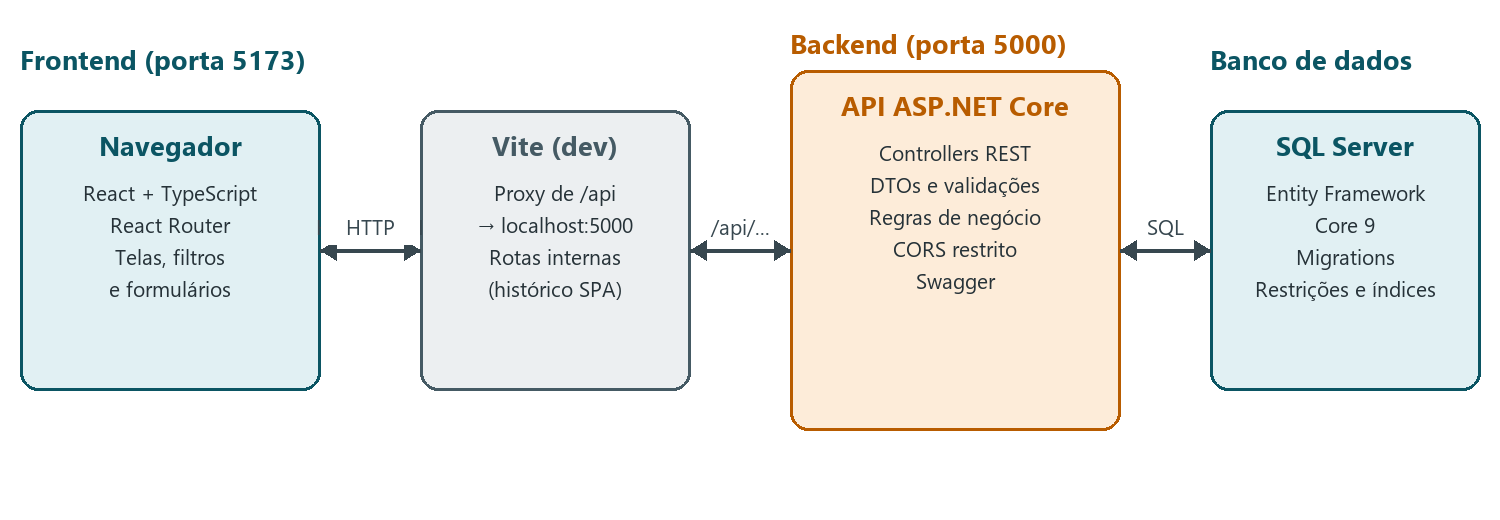
\includegraphics[width=14.4cm]{imagens/arquitetura.png}
  \caption{Arquitetura da solução: frontend, proxy de desenvolvimento, API e banco de dados.}
  \label{fig:arquitetura}
\end{figure}

\begin{table}[H]
  \centering
  \caption{Tecnologias utilizadas.}
  \label{tab:tecnologias}
  \small
  \begin{tabular}{|>{\raggedright\arraybackslash}p{2.35cm}|>{\raggedright\arraybackslash}p{11.55cm}|}
  \hline
  \textbf{Camada} & \textbf{Tecnologias e finalidade} \\ \hline
  Banco & SQL Server; migrations do EF Core; índices únicos e restrições CHECK \\ \hline
  Backend & .NET 9, ASP.NET Core, EF Core 9, controllers REST, Swagger (Swashbuckle) \\ \hline
  Frontend & React 19 \cite{react}, TypeScript 6, Vite 8 \cite{vite}, React Router 7 \cite{router}, \texttt{fetch} e CSS próprio \\ \hline
  Testes & Vitest 5 \cite{vitest} e Testing Library \cite{rtl} (telas e serviços); Playwright \cite{playwright} e axe-core \cite{axe} (ponta a ponta e acessibilidade) \\ \hline
  Qualidade & ESLint (com regras de hooks do React) e verificador de tipos do TypeScript em modo estrito \\ \hline
  \end{tabular}
\end{table}

Foram evitadas bibliotecas desnecessárias: não há biblioteca de componentes visuais, de gerenciamento de estado ou de requisições. A identidade visual (azul-petróleo com destaque laranja, logotipo e ícones de traço) foi criada para este projeto, sem imagens ou textos de terceiros.

\section{Wireframes}

Antes de programar, foram desenhados 20 wireframes de alta fidelidade em formato desktop (1440 px), que cobrem: layout e navegação; painel inicial; lista e formulário de cada entidade; as consultas de clientes sem aluguéis, veículos disponíveis, veículos por fabricante, aluguéis por período e histórico por cliente; a janela de devolução; a confirmação de exclusão; e os estados de carregamento, lista vazia, erro e avisos. Cada quadro traz anotações numeradas e uma faixa de notas que relaciona a tela às rotas da API.

Os quadros são gerados por um script (\texttt{npm run wireframes}) a partir de descrições de layout e exportados em SVG editável e PNG, o que permite recriá-los de forma consistente sempre que uma tela mudar. As imagens PNG estão em \texttt{docs/\allowbreak{}wireframes/\allowbreak{}} e os arquivos SVG editáveis em \texttt{docs/\allowbreak{}wireframes/\allowbreak{}svg/\allowbreak{}}.

Os 20 wireframes estão disponíveis \textbf{no Figma}, em \textbf{PNG} e em \textbf{SVG editável}. O arquivo do Figma pode ser acessado em:

\url{https://www.figma.com/design/h5DPiA2ZDKuXXmZ4pPTxMg/Untitled?node-id=1-3&t=qwLSrYq5Za5AQfFy-1}

\begin{figure}[H]
  \centering
  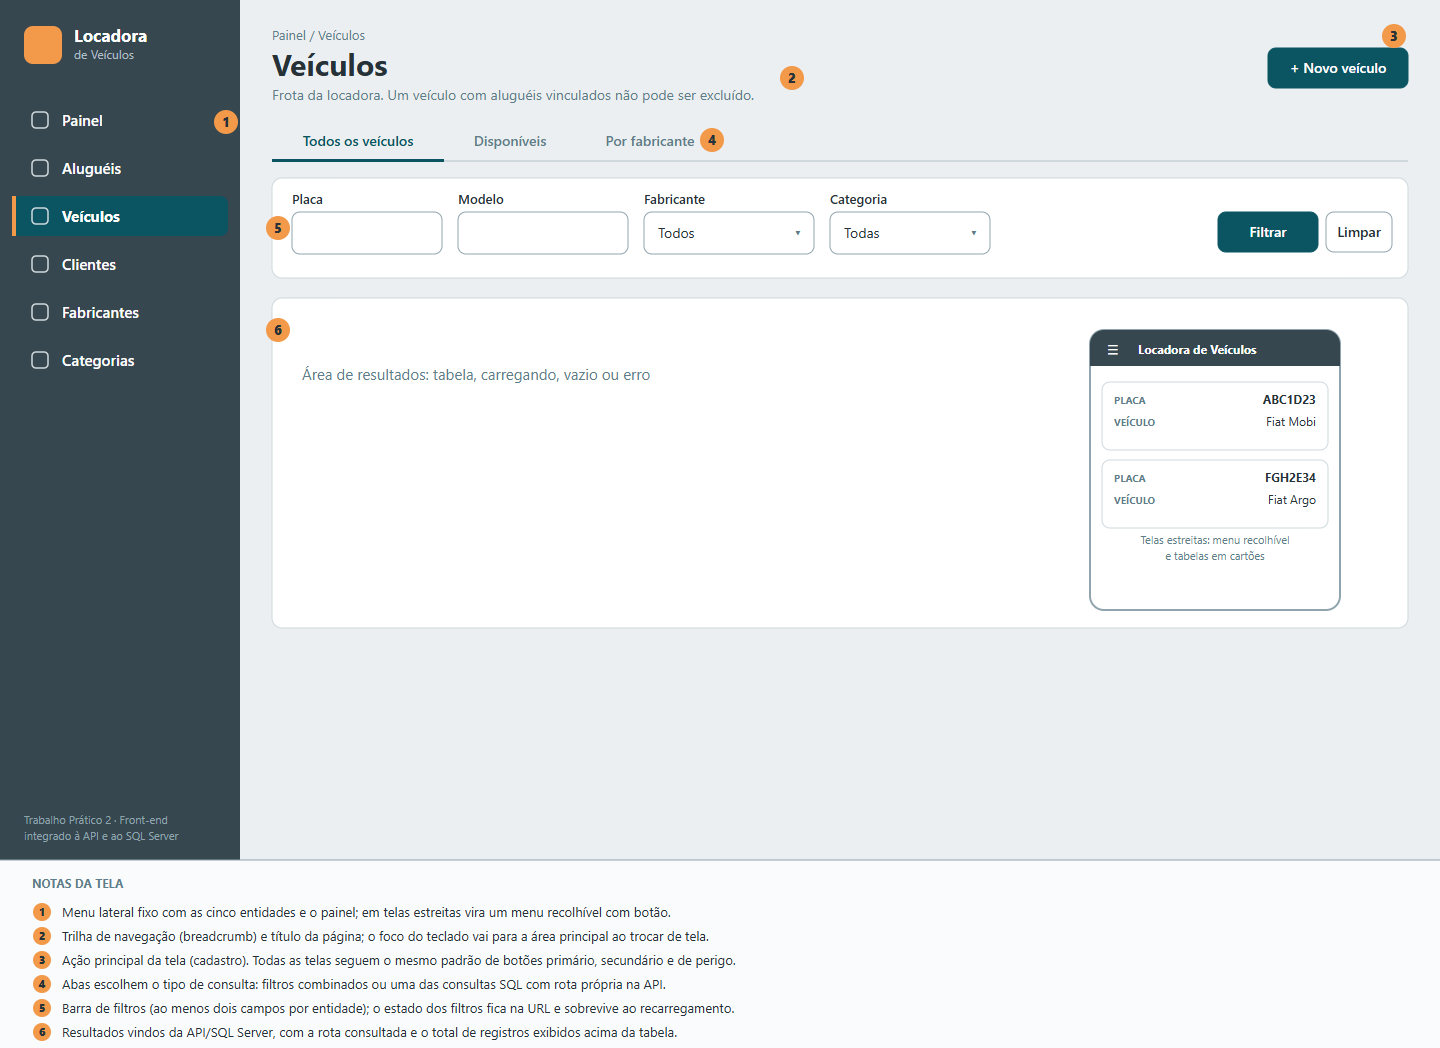
\includegraphics[width=11.5cm]{imagens/wf-layout.png}
  \caption{Wireframe do layout geral e da navegação (menu, trilha, abas, filtros e resultados), com esboço da versão móvel.}
  \label{fig:wflayout}
\end{figure}

\begin{figure}[H]
  \centering
  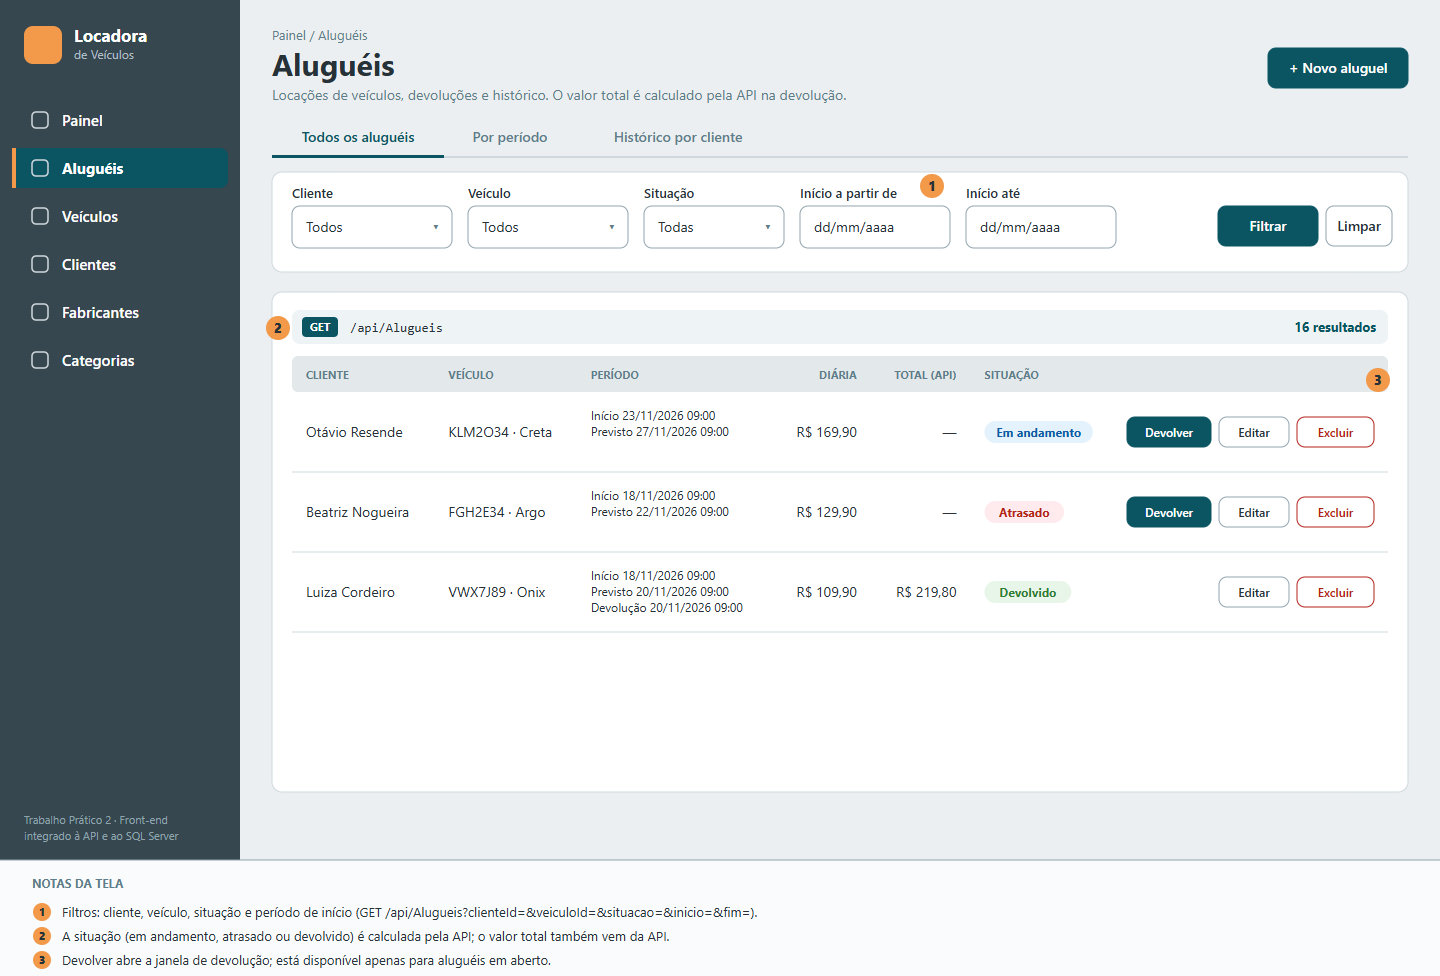
\includegraphics[width=11.5cm]{imagens/wf-alugueis-lista.png}
  \caption{Wireframe da listagem de aluguéis, que foi seguido na tela implementada (Figura~\ref{fig:telaalugueis}).}
  \label{fig:wfalugueis}
\end{figure}

\begin{table}[H]
  \centering
  \caption{Correspondência entre wireframes e telas implementadas.}
  \label{tab:wftelas}
  \small
  \begin{tabular}{|>{\raggedright\arraybackslash}p{4.19cm}|>{\raggedright\arraybackslash}p{5.59cm}|>{\raggedright\arraybackslash}p{3.67cm}|}
  \hline
  \textbf{Wireframe} & \textbf{Tela / rota} & \textbf{Captura} \\ \hline
  01 Painel & \texttt{/\allowbreak{}} & Figura~\ref{fig:telapainel} \\ \hline
  02–05 Fabricantes e categorias & \texttt{/\allowbreak{}fabricantes}, \texttt{/\allowbreak{}categorias} (lista, novo, editar) & Figura~\ref{fig:telavalidacao}, Figura~\ref{fig:telaconfirmar} \\ \hline
  06–08 Clientes & \texttt{/\allowbreak{}clientes} (aba Sem aluguéis), \texttt{/\allowbreak{}clientes/\allowbreak{}novo} & Figura~\ref{fig:telaclientes}, Figura~\ref{fig:telaclienteform} \\ \hline
  09–11 e 18 Veículos & \texttt{/\allowbreak{}veiculos} (abas Disponíveis e Por fabricante) & Figura~\ref{fig:telaveiculosfiltros}, Figura~\ref{fig:telaveiculos} \\ \hline
  12–14, 19 Aluguéis & \texttt{/\allowbreak{}alugueis} (abas Por período e Histórico por cliente) & Figura~\ref{fig:telaalugueis}, Figura~\ref{fig:telaperiodo} \\ \hline
  15 Devolução; 16 Exclusão; 17 Estados & Janelas e avisos compartilhados & Figura~\ref{fig:teladevolucao}, Figura~\ref{fig:telaapi} \\ \hline
  \end{tabular}
\end{table}

\section{Implementação das telas}

\subsection{Layout, navegação e painel}

Todas as telas usam o mesmo layout: menu lateral com as cinco entidades e o painel, cabeçalho com trilha de navegação e título, ação principal à direita e área de conteúdo. Em telas estreitas o menu vira um painel recolhível acionado por botão e as tabelas se transformam em cartões. O painel inicial (Figura~\ref{fig:telapainel}) exibe indicadores calculados com listas reais da API (fabricantes, categorias, clientes, veículos, veículos disponíveis, aluguéis em andamento e atrasados), atalhos de cadastro, os aluguéis em aberto e atalhos para as consultas.

\begin{figure}[H]
  \centering
  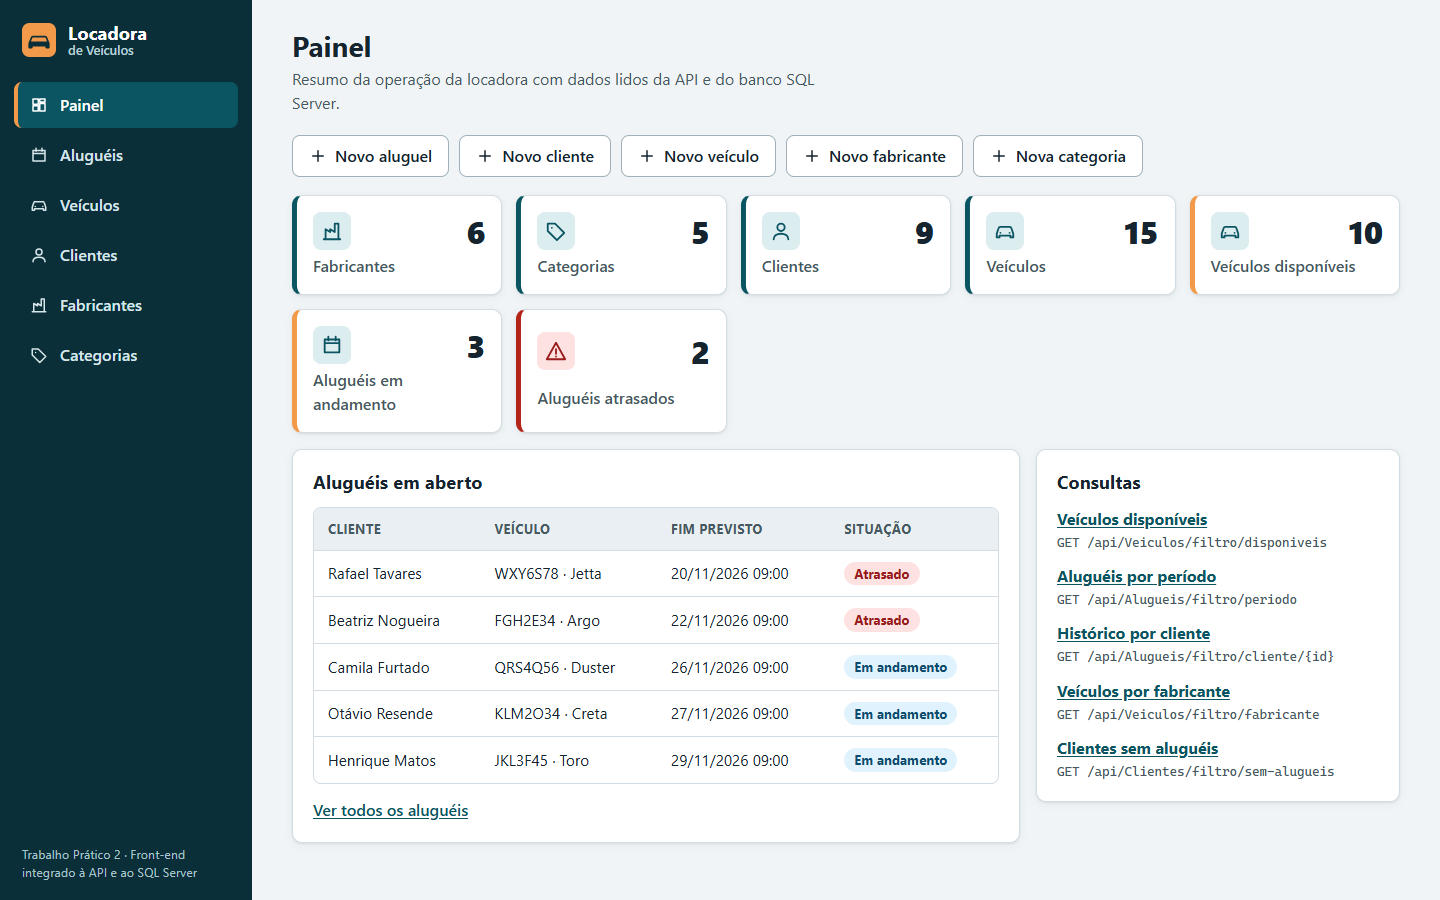
\includegraphics[width=11.5cm]{imagens/tela-painel.png}
  \caption{Painel inicial com indicadores lidos da API e do SQL Server.}
  \label{fig:telapainel}
\end{figure}

\subsection{Componentes e padrões}

A interface é composta por componentes reutilizáveis: botões, campos com rótulo e mensagem de erro associados, tabela responsiva, selos de situação, abas de consulta, barra de filtros, diálogos modais (elemento nativo \texttt{<dialog>} \cite{mdndialog}), avisos de sucesso e erro e estados de carregamento, vazio e erro. As cinco entidades seguem o mesmo padrão; fabricantes e categorias, por terem apenas o campo nome, compartilham os mesmos componentes de lista e formulário.

\subsection{Acessibilidade e responsividade}

Foram adotadas práticas das diretrizes WCAG 2.2 \cite{wcag}: rótulos associados a cada campo, resumo de erros com \texttt{role=\textquotedbl{}alert\textquotedbl{}} e foco movido para ele, foco visível, navegação por teclado, link para pular ao conteúdo, foco devolvido à área principal a cada troca de tela, contraste adequado e respeito à preferência por menos movimento. Uma varredura automática com axe-core nas sete telas principais não encontrou violações graves ou críticas dos níveis A e AA (Seção 12). A responsividade foi verificada em largura de celular (Figura~\ref{fig:telamobile}).

\begin{figure}[H]
  \centering
  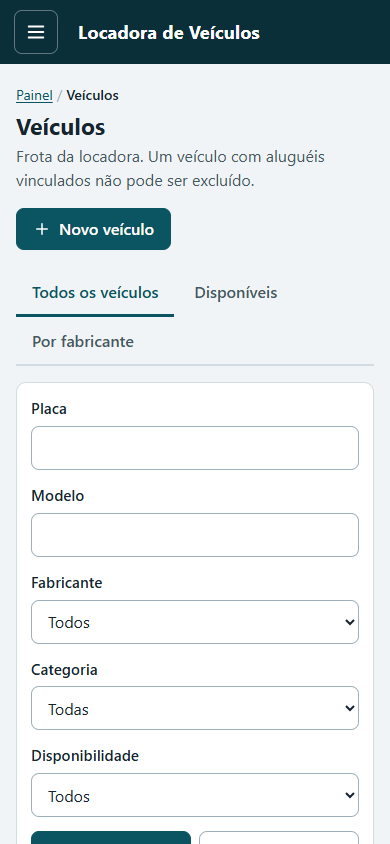
\includegraphics[width=5.2cm]{imagens/tela-mobile.png}
  \caption{Tela de veículos em largura de celular: menu recolhível e filtros empilhados.}
  \label{fig:telamobile}
\end{figure}

\section{Integração com a API}

\subsection{Camada de serviços}

Todo o acesso à API fica em \texttt{frontend/\allowbreak{}src/\allowbreak{}services}. Um cliente HTTP único (\texttt{http.\allowbreak{}ts}) monta a URL com base em \texttt{VITE\_\allowbreak{}API\_\allowbreak{}URL} (vazia por padrão, para usar o proxy do Vite), serializa o JSON e converte as respostas em dados ou em um erro tipado (\texttt{ApiError}). Cada entidade tem um módulo com as operações REST e com as rotas especiais, e uma função gera a lista de operações padrão (obter, criar, atualizar, excluir), evitando repetição.

\subsection{Tratamento de respostas e erros}

O cliente trata \texttt{200}, \texttt{201}, \texttt{204}, \texttt{400}, \texttt{404}, \texttt{409} e \texttt{500}, além de falha de rede, API indisponível e JSON inválido. Respostas \texttt{400} no formato \texttt{ValidationProblemDetails} são convertidas em mensagens por campo (as chaves vêm em PascalCase no corpo e em camelCase na query string, e são normalizadas); mensagens \texttt{\{ \textquotedbl{}mensagem\textquotedbl{}: .\allowbreak{}.\allowbreak{}.\allowbreak{} \}} são exibidas como estão. Um erro \texttt{5xx} sem corpo JSON, típico do proxy sem API, vira “Não foi possível conectar à API” (Figura~\ref{fig:telaapi}). Os componentes oferecem a ação “Tentar novamente”.

\begin{figure}[H]
  \centering
  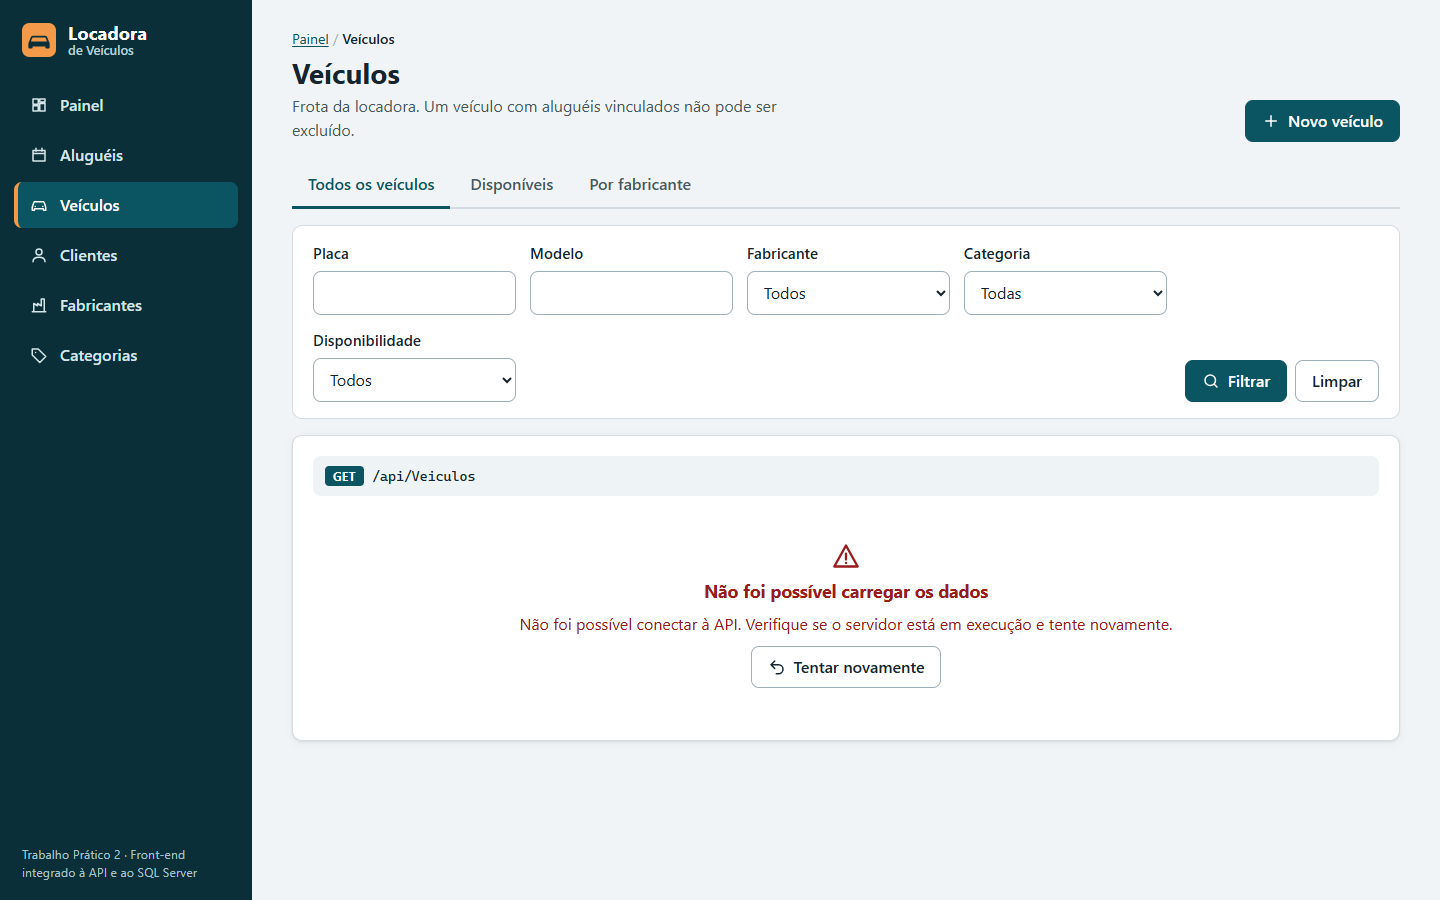
\includegraphics[width=11.0cm]{imagens/tela-api-indisponivel.png}
  \caption{Mensagem exibida quando a API está indisponível, com opção de tentar novamente.}
  \label{fig:telaapi}
\end{figure}

\subsection{Alterações mínimas no backend}

Para a integração foram feitas somente alterações aditivas, sem quebrar o contrato da Etapa 1 e sem alterar o esquema do banco:

\begin{enumerate}
  \item \textbf{CORS restrito} às origens configuradas em \texttt{Cors:AllowedOrigins} (por padrão \texttt{localhost} e \texttt{127.\allowbreak{}0.\allowbreak{}0.\allowbreak{}1} nas portas 5173 e 4173), com os métodos GET, POST, PUT e DELETE e o cabeçalho \texttt{Content-Type} \cite{cors}. Como o tratador global de exceções limpa os cabeçalhos da resposta, a política é reaplicada nele para que o navegador consiga ler as mensagens \texttt{409} e \texttt{500};
  \item \textbf{filtros opcionais por query string} nos \texttt{GET} de listagem (por exemplo \texttt{GET /\allowbreak{}api/\allowbreak{}Veiculos?placa=abc\&disponivel=true}), de modo que o filtro seja executado no banco e não no navegador;
  \item \textbf{campos derivados}: \texttt{disponivel} nas respostas de veículo e \texttt{situacao} (\texttt{EmAndamento}, \texttt{Atrasado} ou \texttt{Devolvido}) nas de aluguel, calculados na consulta;
  \item O \texttt{.\allowbreak{}csproj} passou a ignorar a pasta \texttt{frontend/\allowbreak{}} na compilação e o \texttt{dotnet-ef} foi registrado como ferramenta local do projeto.
\end{enumerate}

\section{Operações CRUD}

As cinco entidades possuem listagem, cadastro, edição e exclusão, com carregamento, estado vazio, validação de formulário, mensagem de sucesso ou erro e atualização da lista após cada alteração. A validação no navegador espelha as regras da API apenas para dar retorno imediato; as mensagens da API continuam sendo exibidas no formulário quando ocorrem.

\begin{figure}[H]
  \centering
  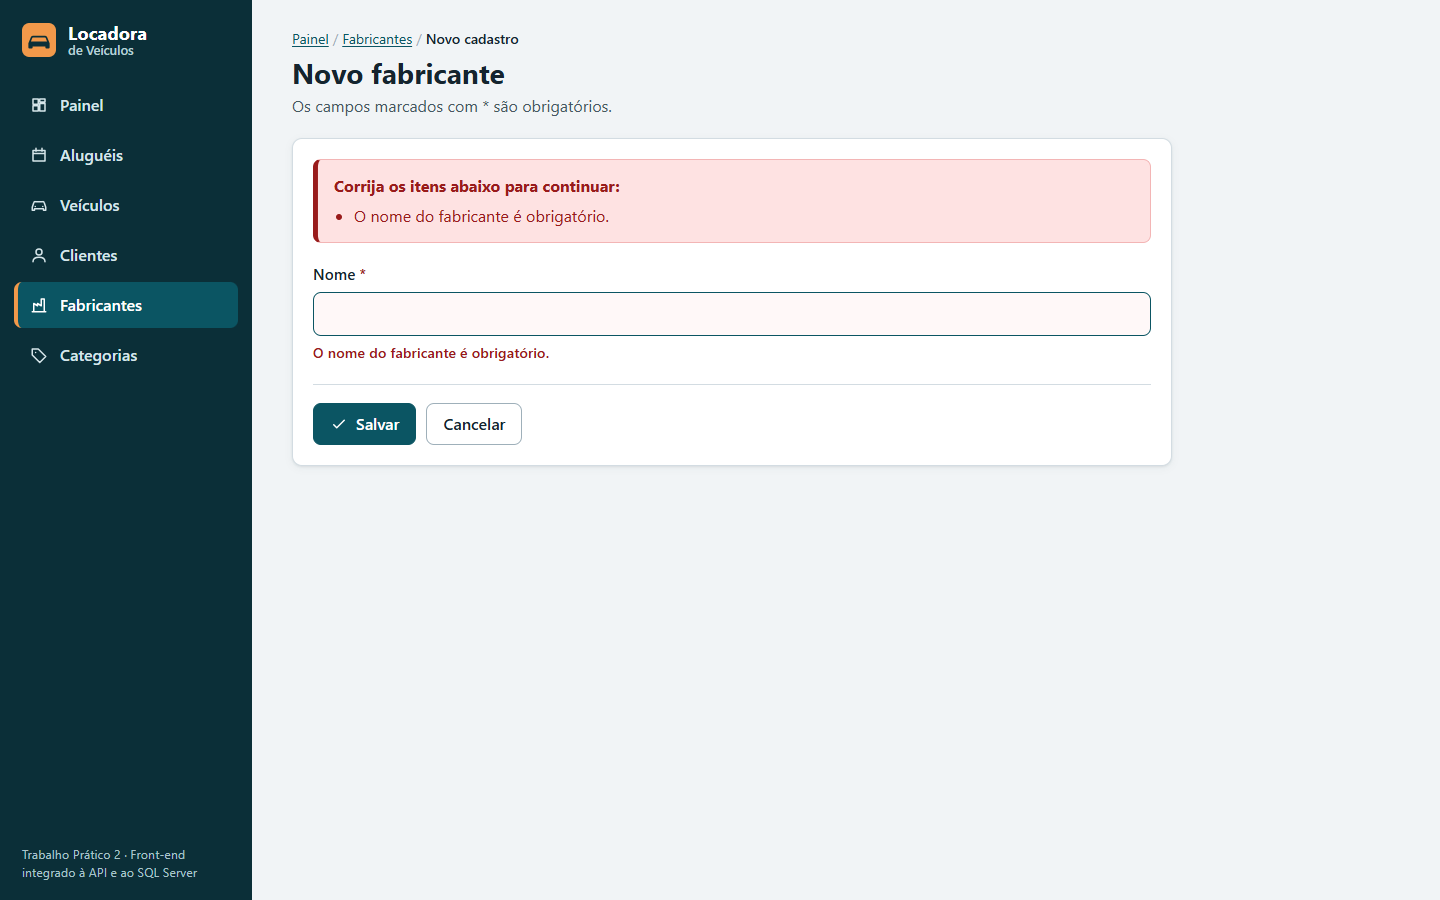
\includegraphics[width=11.0cm]{imagens/tela-validacao.png}
  \caption{Validação de formulário: o resumo de erros recebe o foco e o campo é marcado como inválido.}
  \label{fig:telavalidacao}
\end{figure}

\begin{itemize}
  \item \textbf{Fabricantes e categorias:} formulário com o campo nome; exclusão recusada com \texttt{409} quando há veículos vinculados.
  \item \textbf{Clientes:} nome, CPF com máscara (000.000.000-00; a API recebe apenas os 11 dígitos) e e-mail; CPF ou e-mail duplicados retornam \texttt{409} (Figura~\ref{fig:telaclienteform}).
  \item \textbf{Veículos:} placa (ABC1234, ABC-1234 ou ABC1D23), modelo, ano, quilometragem e seleção de fabricante e categoria carregados da API.
  \item \textbf{Aluguéis:} cliente e veículo carregados da API (em um novo aluguel, apenas veículos disponíveis pela rota \texttt{/\allowbreak{}filtro/\allowbreak{}disponiveis}), datas, quilometragens e diária; o valor total é sempre o retornado pela API.
\end{itemize}

\begin{figure}[H]
  \centering
  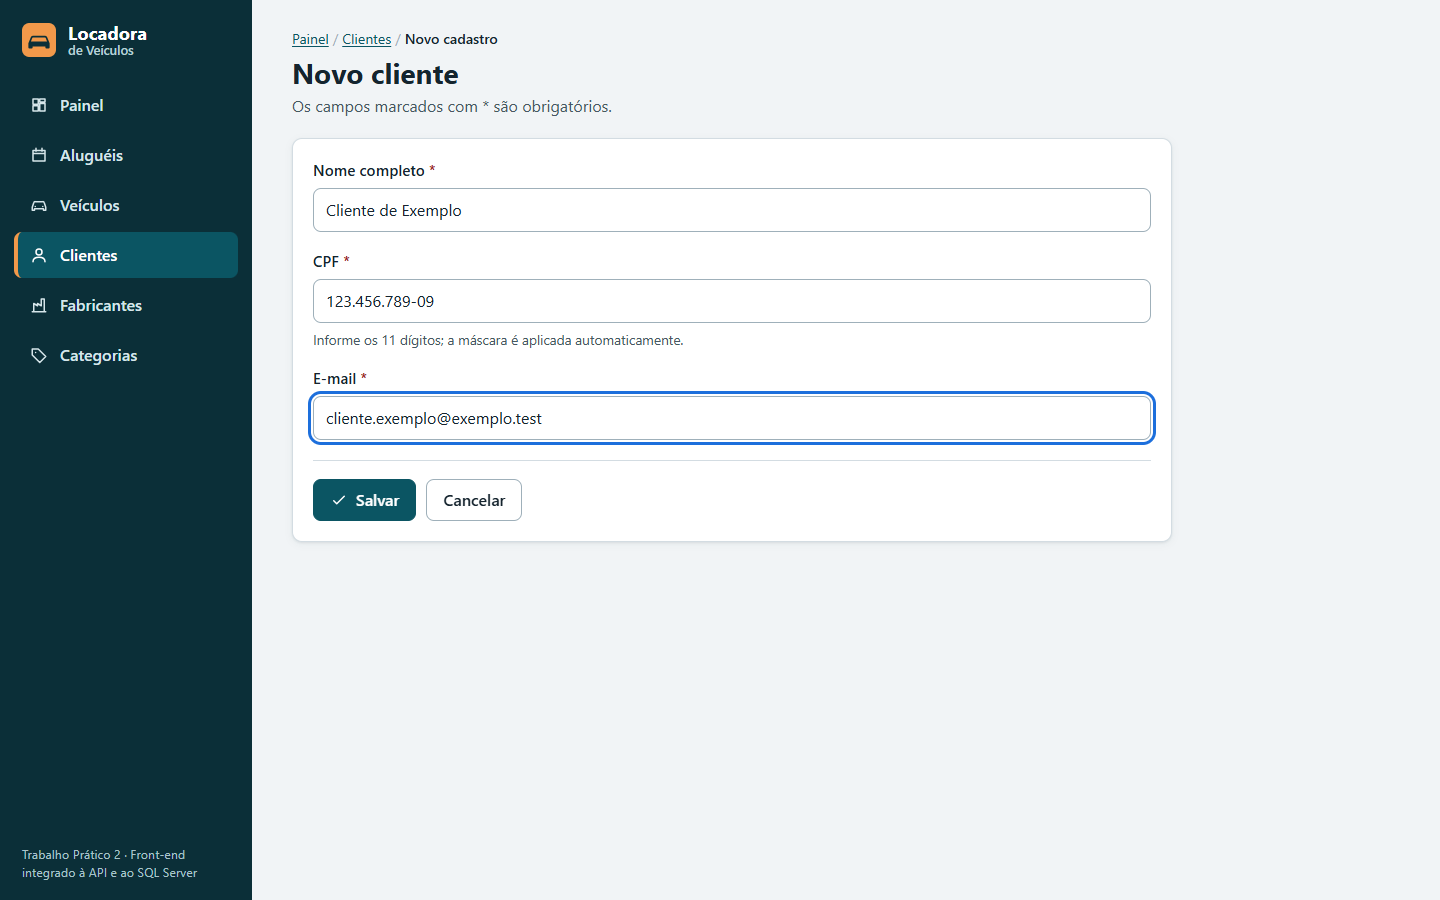
\includegraphics[width=11.0cm]{imagens/tela-clientes-form.png}
  \caption{Formulário de cliente com CPF formatado automaticamente.}
  \label{fig:telaclienteform}
\end{figure}

Toda exclusão pede confirmação em um diálogo modal (Figura~\ref{fig:telaconfirmar}). Se a API recusar por vínculos, a mensagem de conflito aparece em um aviso e nada é alterado (Figura~\ref{fig:tela409}). A ordem de exclusão respeita as chaves estrangeiras: aluguéis, veículos, clientes e, por fim, categorias e fabricantes.

\begin{figure}[H]
  \centering
  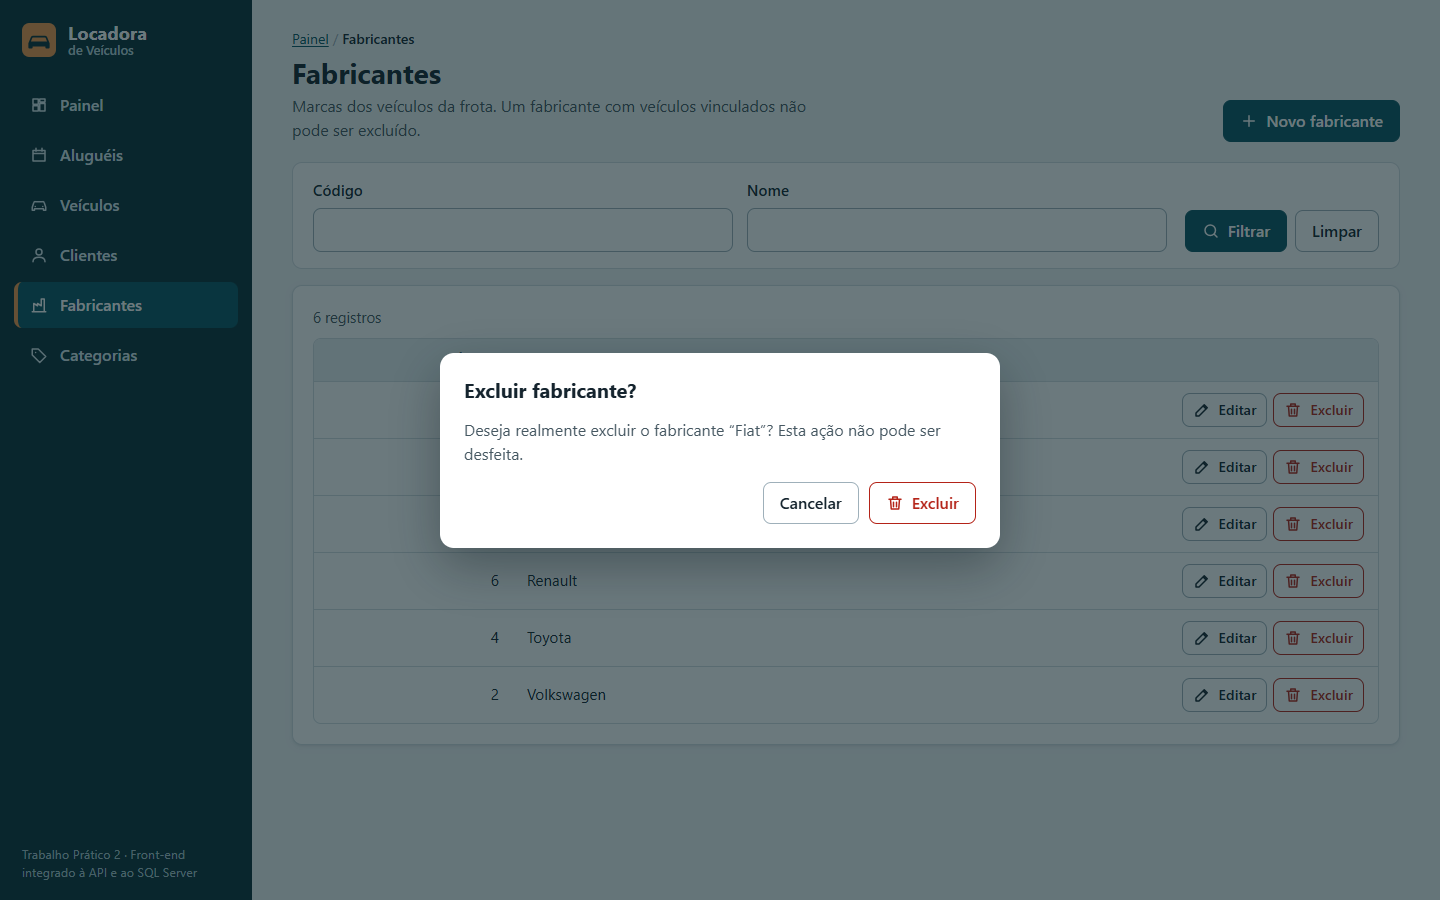
\includegraphics[width=11.0cm]{imagens/tela-confirmar-exclusao.png}
  \caption{Confirmação antes de excluir um registro.}
  \label{fig:telaconfirmar}
\end{figure}

\begin{figure}[H]
  \centering
  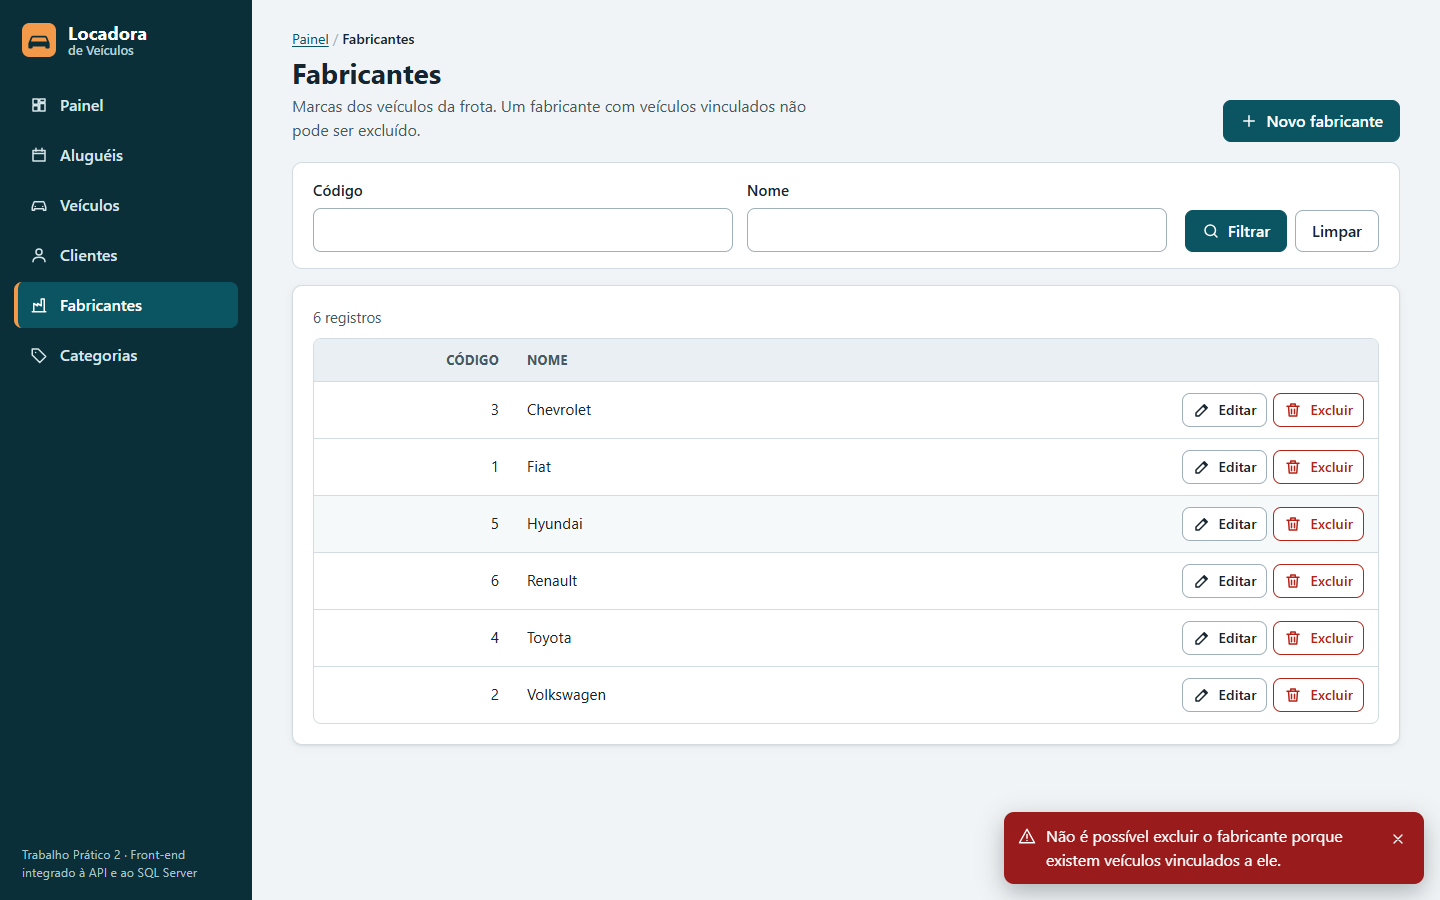
\includegraphics[width=11.0cm]{imagens/tela-conflito-409.png}
  \caption{Conflito 409: o fabricante possui veículos vinculados e não pode ser excluído.}
  \label{fig:tela409}
\end{figure}

\subsection{Registro de devolução}

A API só oferece \texttt{PUT} completo para alterar um aluguel. A janela de devolução (Figura~\ref{fig:teladevolucao}) carrega o aluguel, pede data e hora e quilometragem final e envia o \texttt{PUT} com os dados atuais e a devolução preenchida. Em seguida lê novamente o aluguel e informa o valor total calculado pela API (Figura~\ref{fig:teladevolucaores}). A regra de cobrança fica no backend: cada dia iniciado conta como uma diária, com no mínimo uma. O frontend mostra apenas uma \textbf{estimativa}, identificada como tal, para orientar o usuário antes de confirmar.

\begin{figure}[H]
  \centering
  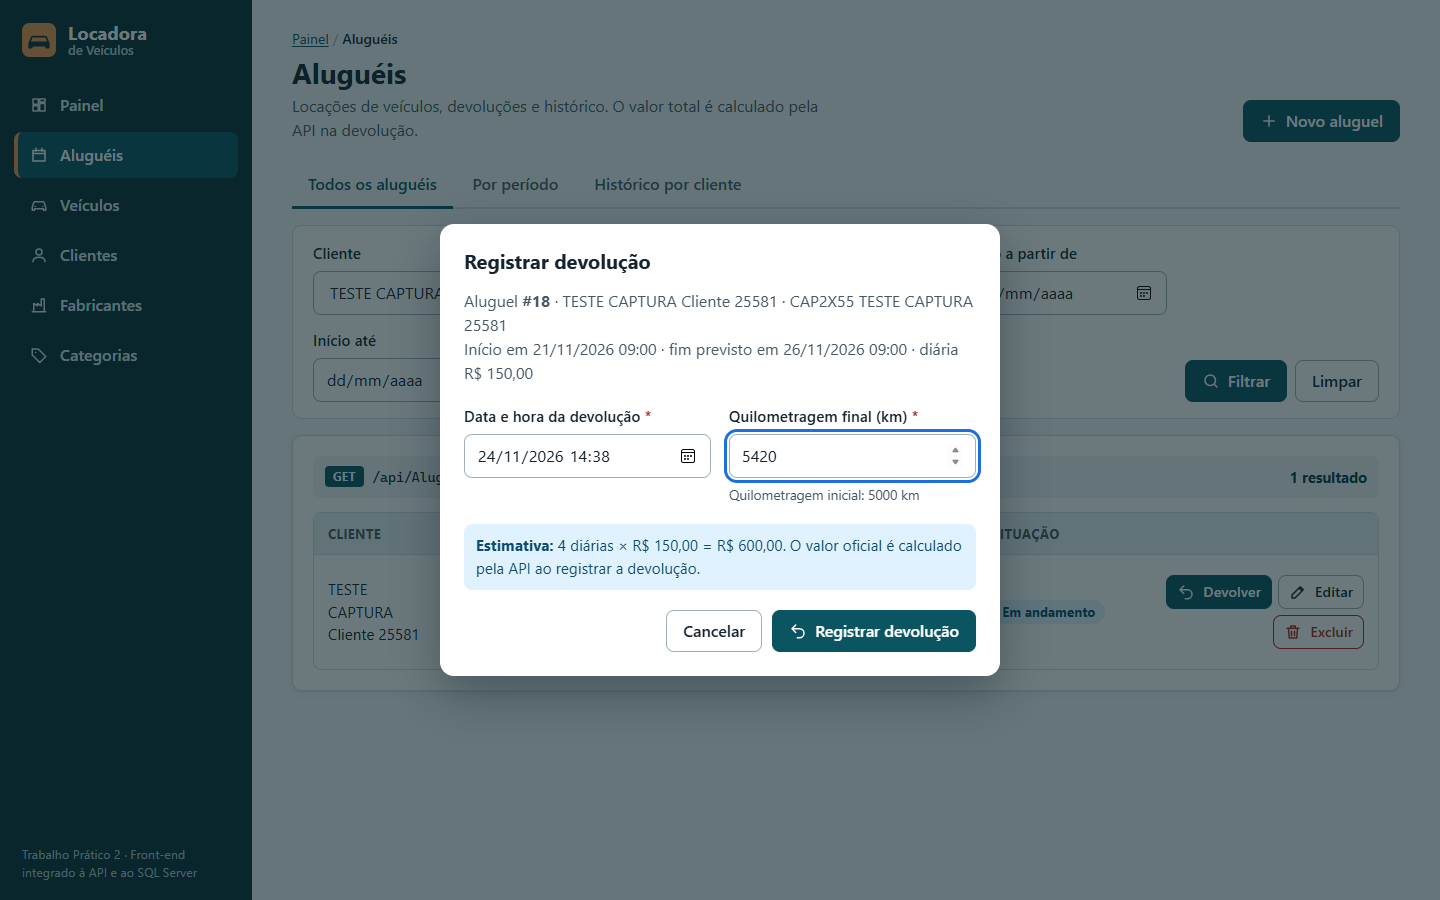
\includegraphics[width=11.0cm]{imagens/tela-devolucao-janela.png}
  \caption{Janela de devolução com estimativa visual identificada como tal.}
  \label{fig:teladevolucao}
\end{figure}

\begin{figure}[H]
  \centering
  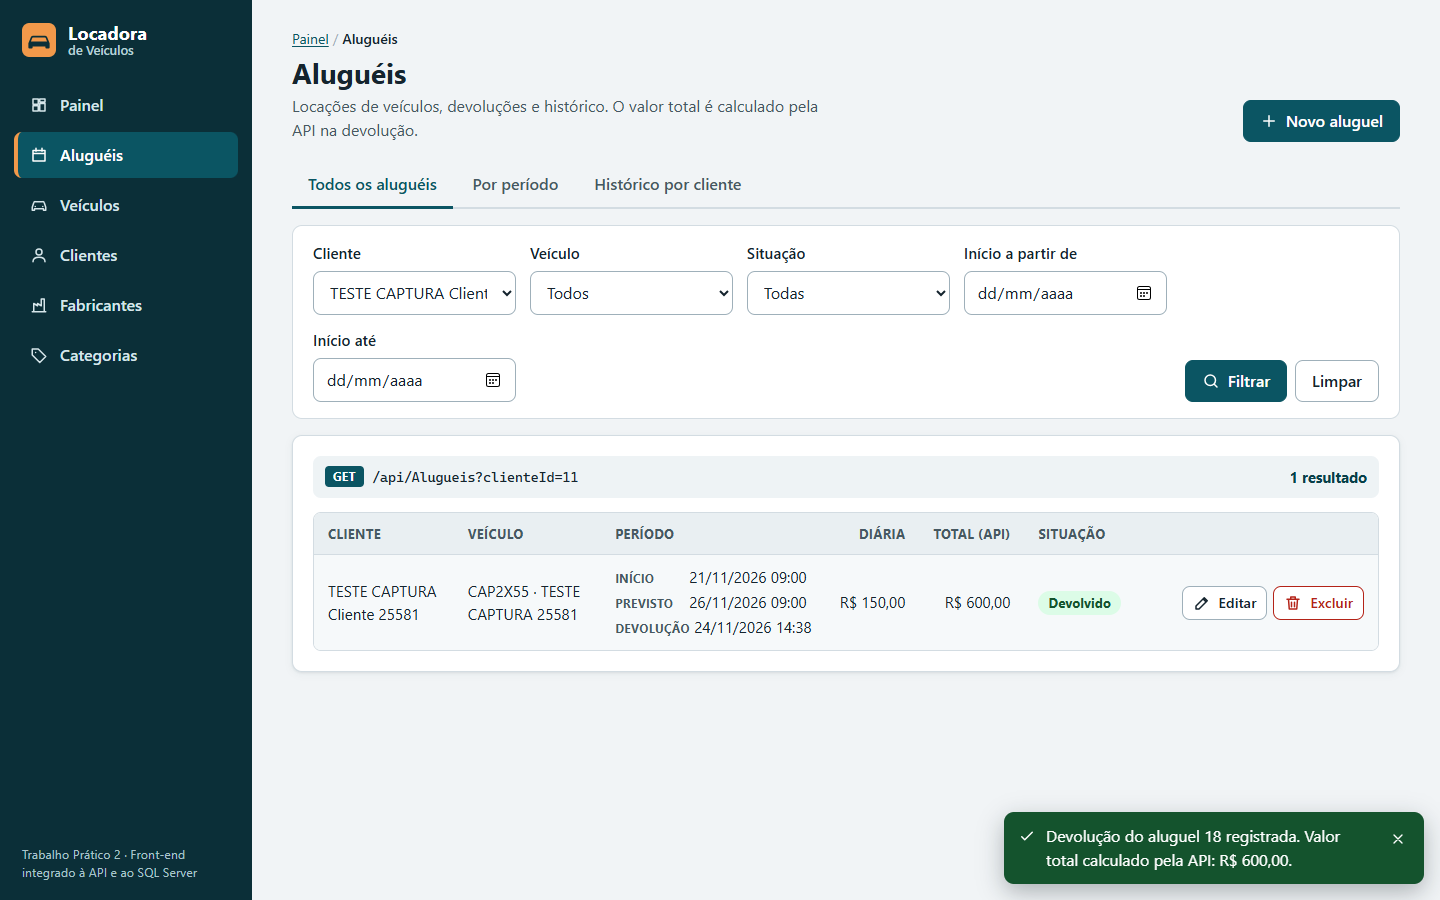
\includegraphics[width=11.0cm]{imagens/tela-devolucao-resultado.png}
  \caption{Resultado da devolução: situação “Devolvido” e valor total calculado pela API (4 diárias de R\$ 150,00).}
  \label{fig:teladevolucaores}
\end{figure}

\section{Filtros}

Cada entidade oferece filtros em pelo menos dois campos (Tabela~\ref{tab:filtros}). O estado dos filtros e o tipo de consulta ficam na URL, o que preserva a consulta ao recarregar a página, ao voltar no histórico e ao compartilhar o link. As consultas com rota própria da Etapa 1 aparecem como abas, que exibem a rota chamada e o total de resultados.

\begin{table}[H]
  \centering
  \caption{Filtros e consultas por entidade.}
  \label{tab:filtros}
  \small
  \begin{tabular}{|>{\raggedright\arraybackslash}p{1.92cm}|>{\raggedright\arraybackslash}p{5.24cm}|>{\raggedright\arraybackslash}p{6.29cm}|}
  \hline
  \textbf{Entidade} & \textbf{Filtros combinados (GET de listagem)} & \textbf{Consultas com rota própria} \\ \hline
  Fabricante & código, nome & — \\ \hline
  Categoria & código, nome & — \\ \hline
  Cliente & nome, CPF, e-mail & \texttt{/\allowbreak{}api/\allowbreak{}Clientes/\allowbreak{}filtro/\allowbreak{}sem-alugueis} \\ \hline
  Veículo & placa, modelo, fabricante, categoria, disponibilidade & \texttt{/\allowbreak{}api/\allowbreak{}Veiculos/\allowbreak{}filtro/\allowbreak{}disponiveis}; \texttt{/\allowbreak{}api/\allowbreak{}Veiculos/\allowbreak{}filtro/\allowbreak{}fabricante?nome=} \\ \hline
  Aluguel & cliente, veículo, situação, data inicial e final & \texttt{/\allowbreak{}api/\allowbreak{}Alugueis/\allowbreak{}filtro/\allowbreak{}periodo?inicio=\&fim=}; \texttt{/\allowbreak{}api/\allowbreak{}Alugueis/\allowbreak{}filtro/\allowbreak{}cliente/\allowbreak{}\{id\}} \\ \hline
  \end{tabular}
\end{table}

\begin{figure}[H]
  \centering
  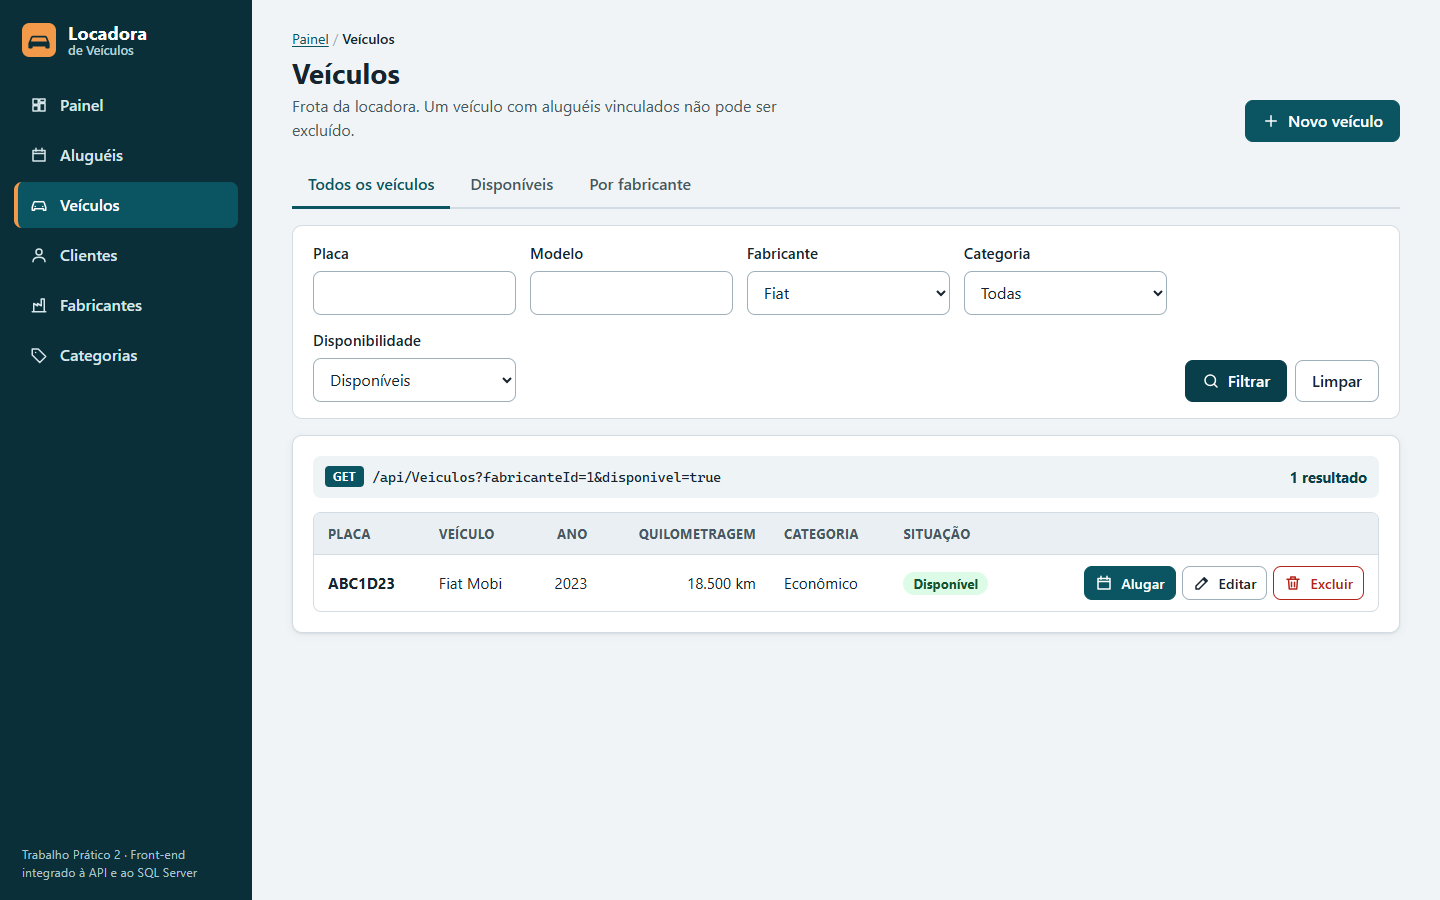
\includegraphics[width=11.0cm]{imagens/tela-veiculos-filtros.png}
  \caption{Filtros combinados em veículos: fabricante e disponibilidade, enviados à API como parâmetros.}
  \label{fig:telaveiculosfiltros}
\end{figure}

\begin{figure}[H]
  \centering
  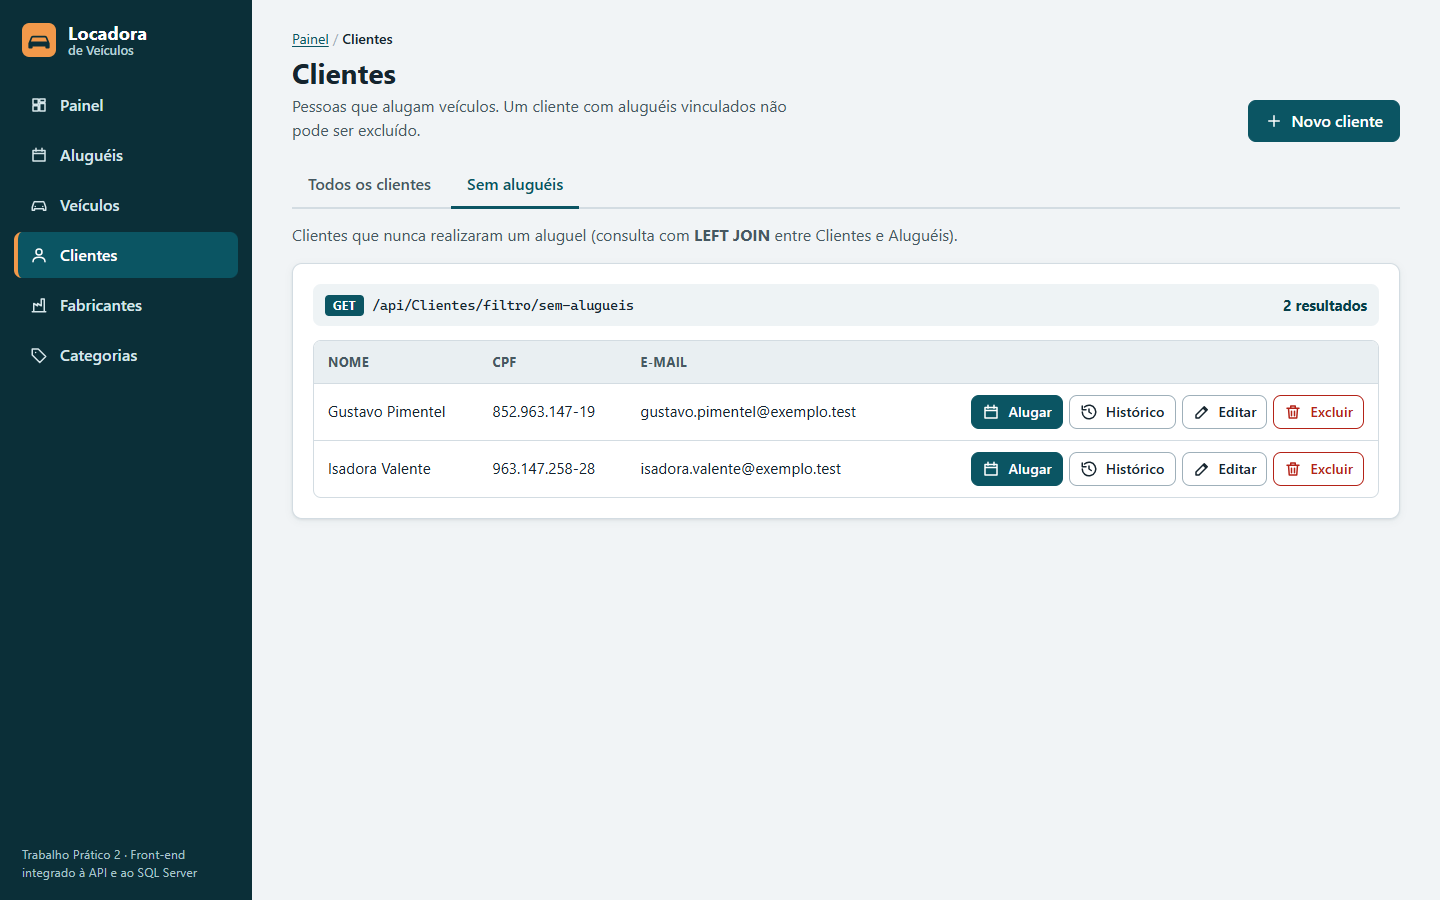
\includegraphics[width=11.0cm]{imagens/tela-clientes-sem-alugueis.png}
  \caption{Clientes sem aluguéis (consulta LEFT JOIN) com a rota exibida.}
  \label{fig:telaclientes}
\end{figure}

\begin{figure}[H]
  \centering
  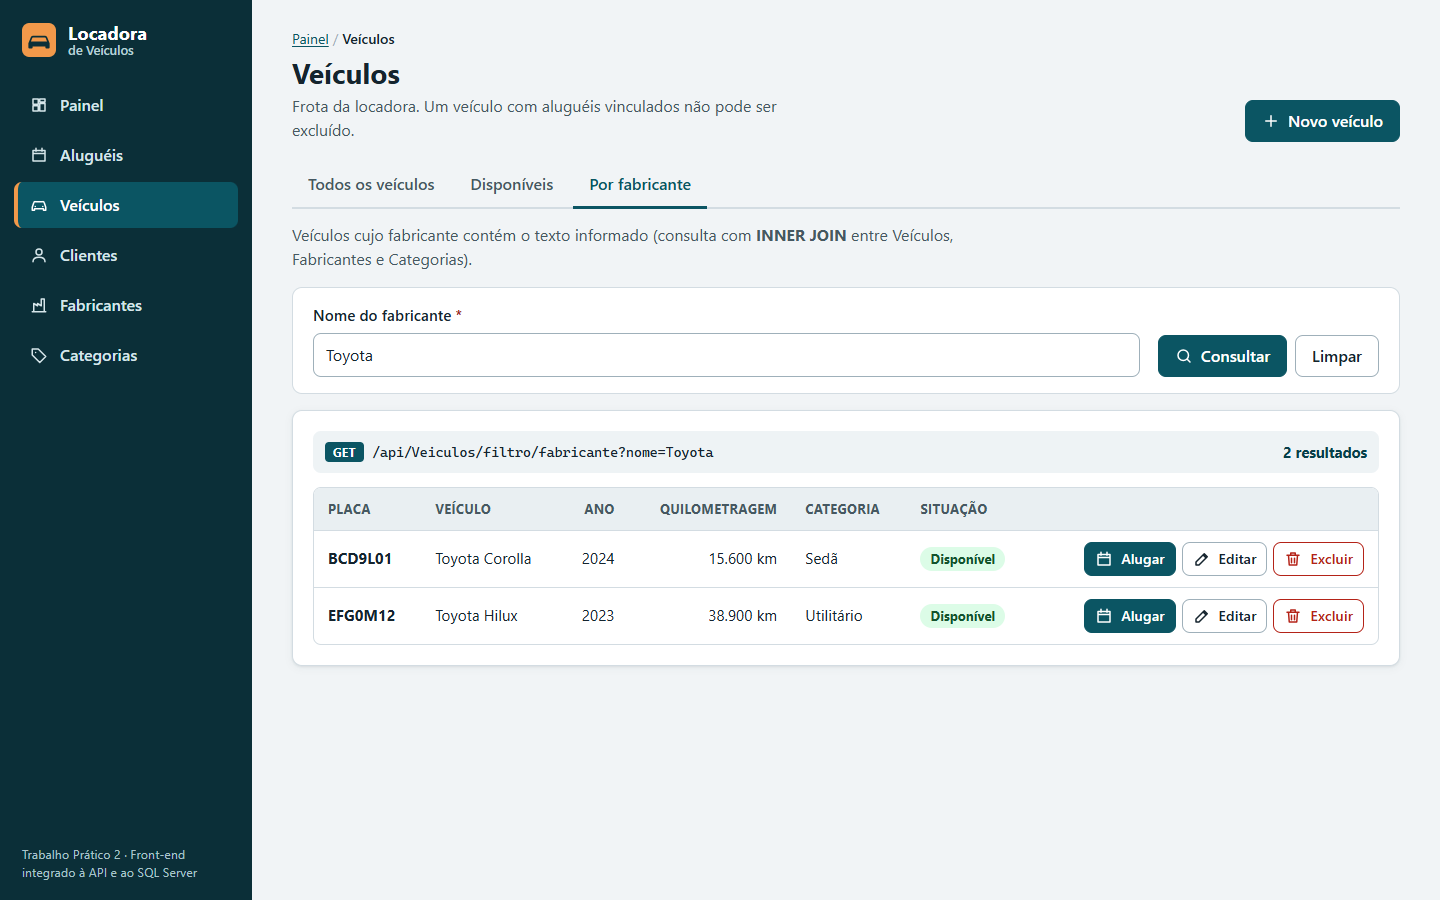
\includegraphics[width=11.0cm]{imagens/tela-veiculos-fabricante.png}
  \caption{Veículos por fabricante (INNER JOIN): rota com o nome informado e resultados.}
  \label{fig:telaveiculos}
\end{figure}

\begin{figure}[H]
  \centering
  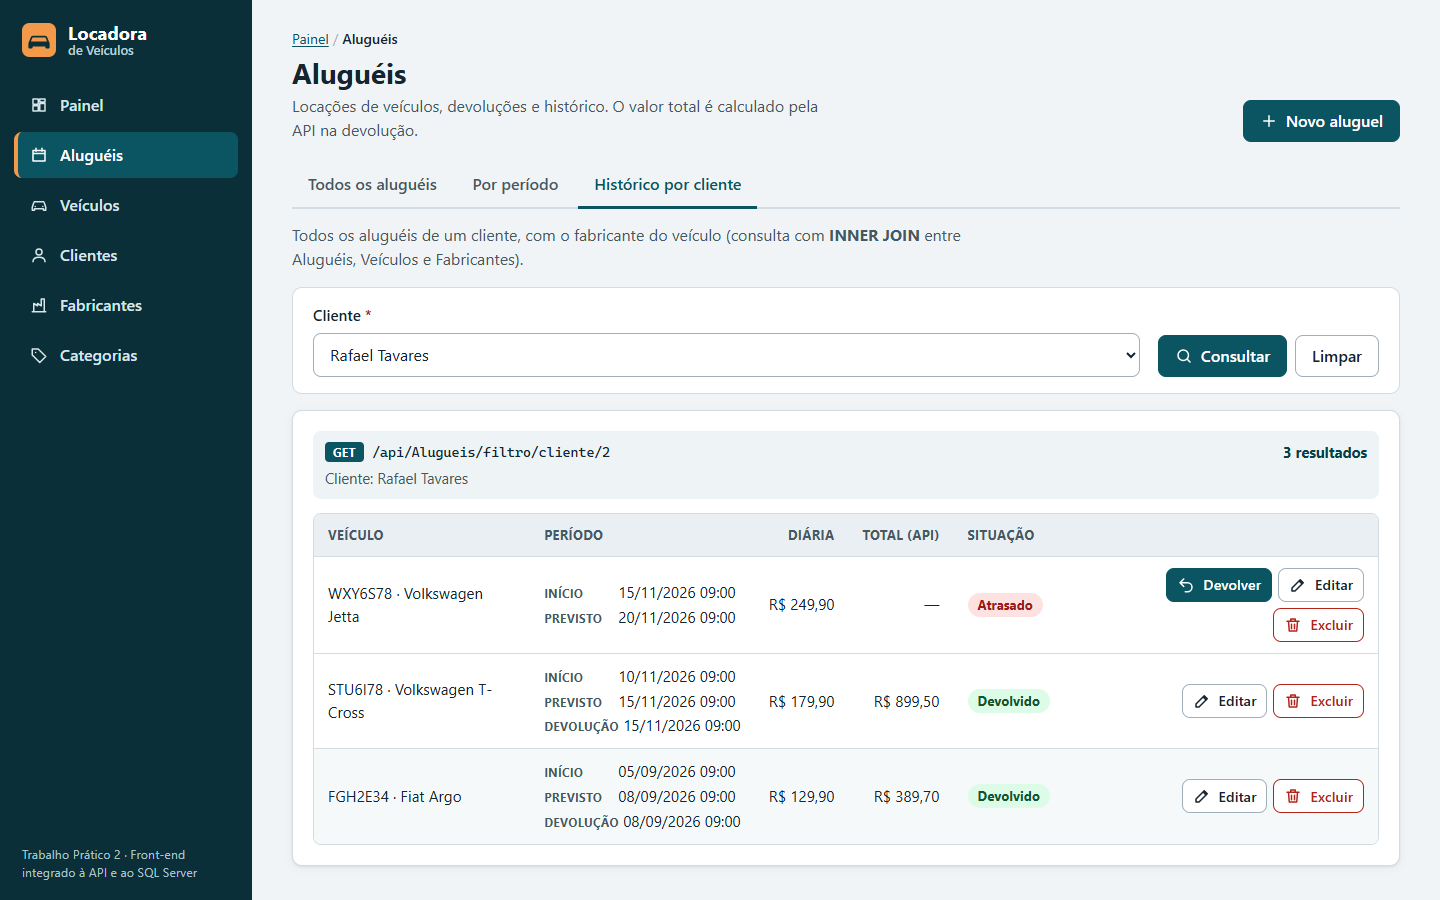
\includegraphics[width=11.0cm]{imagens/tela-alugueis-historico.png}
  \caption{Histórico de aluguéis de um cliente, acessado pelo botão Histórico na lista de clientes.}
  \label{fig:telahistorico}
\end{figure}

\section{Consulta 1: veículos disponíveis}

\textbf{Banco.} Um veículo está disponível quando não existe aluguel em aberto para ele. A consulta faz um \texttt{LEFT JOIN} entre Veículos e os aluguéis sem devolução e mantém as linhas sem correspondência; os \texttt{INNER JOIN} com Fabricantes e Categorias trazem os nomes. Esse é o SQL equivalente ao gerado pelo Entity Framework Core a partir do LINQ do \texttt{VeiculosController}:

{\scriptsize
\begin{verbatim}
SELECT v.Id, v.Placa, v.Modelo, v.AnoFabricacao, v.Quilometragem,
       f.Nome AS Fabricante, c.Nome AS Categoria
FROM Veiculos v
LEFT JOIN Alugueis a ON a.VeiculoId = v.Id AND a.DataDevolucao IS NULL
INNER JOIN Fabricantes f ON f.Id = v.FabricanteId
INNER JOIN Categorias c ON c.Id = v.CategoriaId
WHERE a.Id IS NULL
ORDER BY v.Modelo;
\end{verbatim}
}

\textbf{Rota.} \texttt{GET /\allowbreak{}api/\allowbreak{}Veiculos/\allowbreak{}filtro/\allowbreak{}disponiveis}, que devolve a lista de veículos com o campo \texttt{disponivel} igual a \texttt{true}. \textbf{Chamada do frontend.} A aba Disponíveis da tela de veículos chama \texttt{veiculosApi.\allowbreak{}listarDisponiveis()}, que usa o cliente HTTP central. \textbf{Resultado.} Com os dados de demonstração a consulta retornou 10 veículos, número idêntico ao obtido executando o SQL acima diretamente no SQL Server (Figura~\ref{fig:teladisponiveis}). Após registrar um aluguel para um desses veículos, ele deixa de aparecer na aba, e volta a aparecer após a devolução; esse comportamento é verificado nos testes ponta a ponta.

\begin{figure}[H]
  \centering
  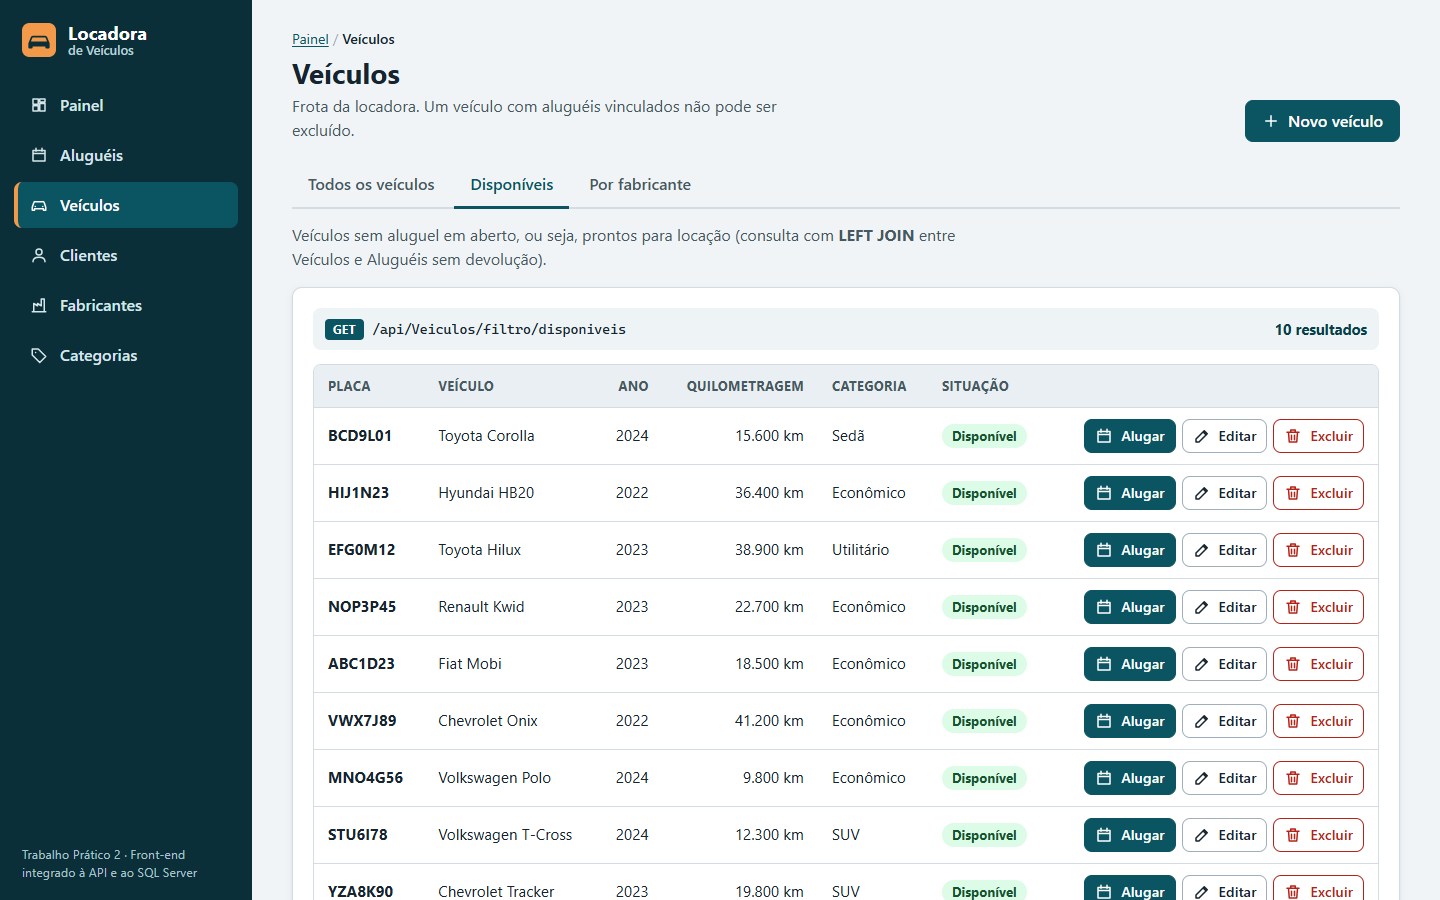
\includegraphics[width=11.5cm]{imagens/tela-veiculos-disponiveis.png}
  \caption{Consulta 1 no frontend: aba Disponíveis, rota chamada e 10 resultados.}
  \label{fig:teladisponiveis}
\end{figure}

\section{Consulta 2: aluguéis por período}

\textbf{Banco.} A consulta lista os aluguéis iniciados dentro de um intervalo, com cliente e veículo, por meio de dois \texttt{INNER JOIN}. A data final é inclusiva; por isso o limite superior da condição é o início do dia seguinte:

{\scriptsize
\begin{verbatim}
SELECT a.Id, c.Nome AS Cliente, v.Placa, v.Modelo, a.DataInicio, a.DataFimPrevista,
       a.DataDevolucao, a.ValorDiaria, a.ValorTotal
FROM Alugueis a
INNER JOIN Clientes c ON c.Id = a.ClienteId
INNER JOIN Veiculos v ON v.Id = a.VeiculoId
WHERE a.DataInicio >= '2026-09-25' AND a.DataInicio < '2026-11-25'
ORDER BY a.DataInicio;
\end{verbatim}
}

\textbf{Rota.} \texttt{GET /\allowbreak{}api/\allowbreak{}Alugueis/\allowbreak{}filtro/\allowbreak{}periodo?inicio=2026-09-25\&fim=2026-11-24}; se a data final for anterior à inicial, a API responde \texttt{400} com uma mensagem, exibida na tela. \textbf{Chamada do frontend.} A aba Por período exige as duas datas e chama \texttt{alugueisApi.\allowbreak{}listarPorPeriodo(inicio, fim)}. \textbf{Resultado.} Para o período de 25/09/2026 a 24/11/2026 a rota retornou 13 aluguéis, o mesmo total do SQL executado no banco (Figura~\ref{fig:telaperiodo}). Cada linha mostra cliente, veículo, datas, situação e o valor total calculado pela API, e permite editar, excluir ou, se estiver em aberto, registrar a devolução.

\begin{figure}[H]
  \centering
  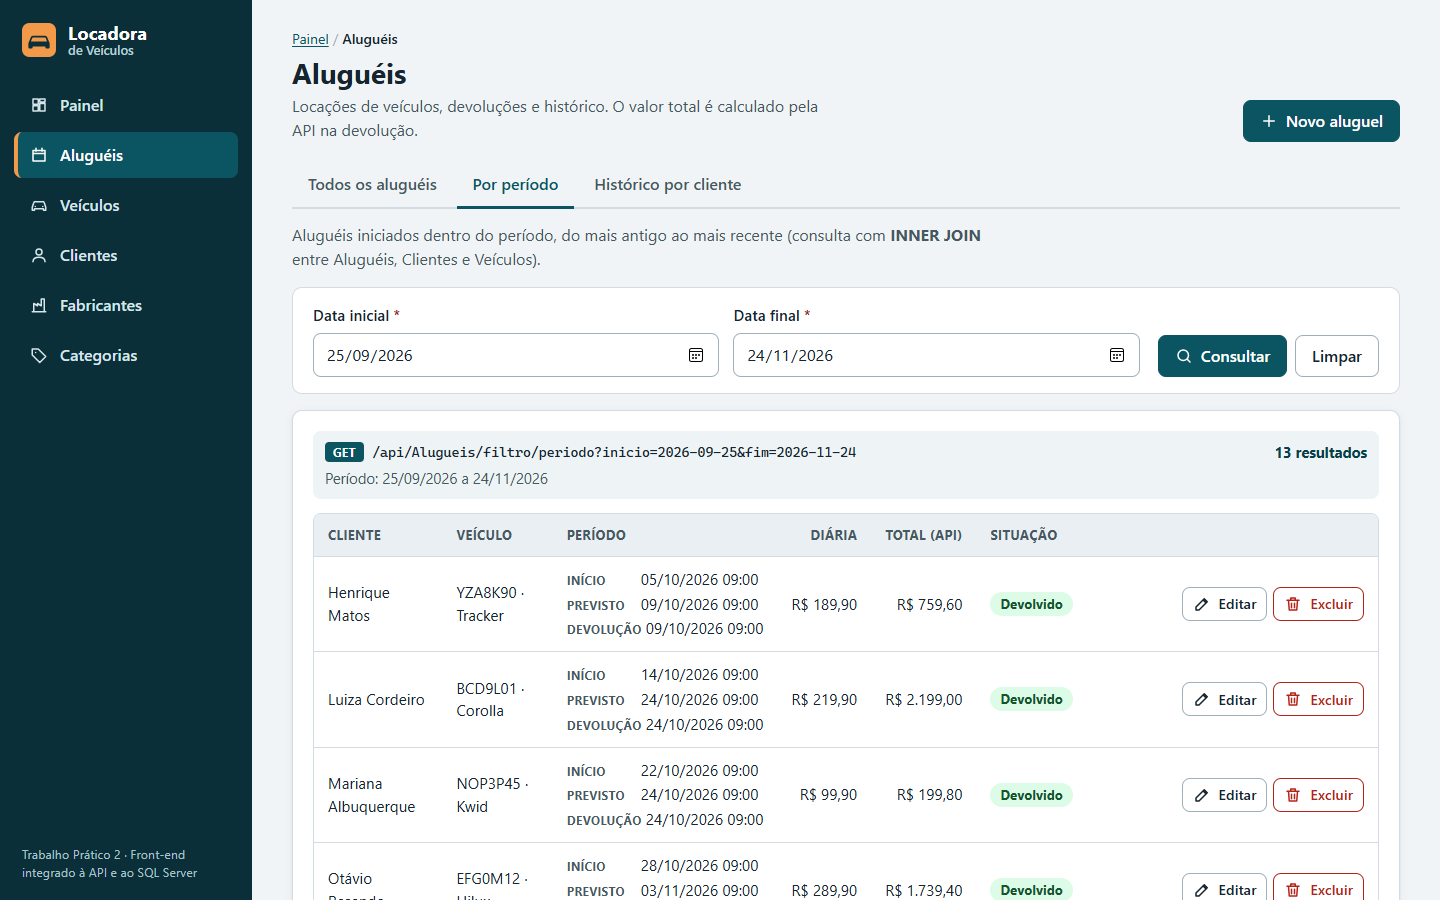
\includegraphics[width=11.5cm]{imagens/tela-alugueis-periodo.png}
  \caption{Consulta 2 no frontend: aluguéis por período, com a rota, o intervalo e 13 resultados.}
  \label{fig:telaperiodo}
\end{figure}

\begin{figure}[H]
  \centering
  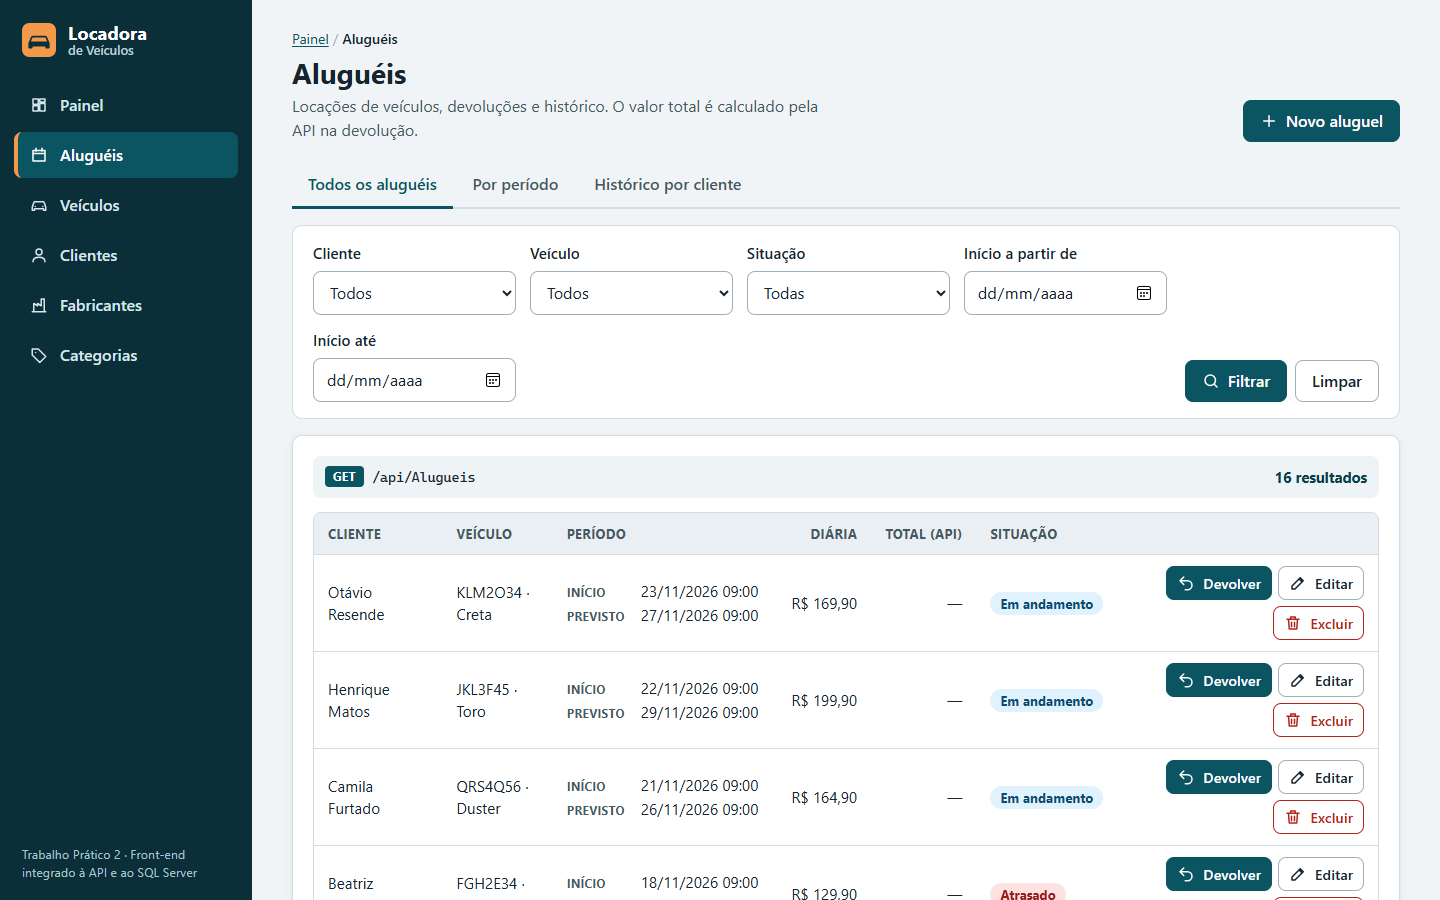
\includegraphics[width=11.5cm]{imagens/tela-alugueis-lista.png}
  \caption{Tela de aluguéis implementada a partir do wireframe da Figura~\ref{fig:wfalugueis}: filtros combinados, situação e ações por linha.}
  \label{fig:telaalugueis}
\end{figure}

\section{Testes e resultados}

Os testes cobrem três níveis. \textbf{Telas e serviços} (Vitest e Testing Library): renderizam a aplicação real com uma API falsa, apenas nos testes, para verificar listagens, filtros, formulários, validações, exclusão com confirmação, conflitos, erros de rede e as consultas especiais (82 testes). \textbf{Ponta a ponta} (Playwright, navegador real, API e SQL Server reais): cadastram, editam, filtram, alugam, devolvem e excluem registros, verificam conflitos \texttt{409}, recarregamento em rotas internas, API indisponível e acessibilidade com axe-core. Os registros criados têm o prefixo “TESTE E2E” e são removidos ao final, o que foi conferido no banco. \textbf{Backend}: compilação sem avisos e conferência manual das rotas contra o banco real, além dos 36 testes pelo Swagger da Etapa 1.

\begin{table}[H]
  \centering
  \caption{Verificações executadas e resultados.}
  \label{tab:testes}
  \small
  \begin{tabular}{|>{\raggedright\arraybackslash}p{4.54cm}|>{\raggedright\arraybackslash}p{4.02cm}|>{\raggedright\arraybackslash}p{4.89cm}|}
  \hline
  \textbf{Verificação} & \textbf{Comando} & \textbf{Resultado} \\ \hline
  Compilação do backend & \texttt{dotnet build} & 0 avisos, 0 erros \\ \hline
  Verificação de tipos & \texttt{npm run typecheck} & sem erros \\ \hline
  Análise estática & \texttt{npm run lint} & sem erros \\ \hline
  Testes de telas e serviços & \texttt{npm test} & 82 aprovados em 7 arquivos \\ \hline
  Build de produção & \texttt{npm run build} & concluído (JS 319,5 kB; 98,0 kB comprimido) \\ \hline
  Ponta a ponta com SQL Server & \texttt{npm run test:e2e} & 8 aprovados (33 a 45 s) \\ \hline
  Acessibilidade (axe-core, A e AA) & dentro do ponta a ponta & 0 violações graves/críticas em 7 telas \\ \hline
  SQL x API & \texttt{sqlcmd} x \texttt{curl} & 10, 13 e 2 linhas, idênticas nas três consultas \\ \hline
  API da Etapa 1 (Swagger) & \texttt{docs/\allowbreak{}relatorio-testes.\allowbreak{}md} & 36 testes aprovados (04/10/2026) \\ \hline
  \end{tabular}
\end{table}

Ambiente: Windows 11, SQL Server 2025 (instância padrão), SDK .NET 10 executando o projeto \texttt{net9.\allowbreak{}0} com \texttt{DOTNET\_\allowbreak{}ROLL\_\allowbreak{}FORWARD}, Node.js 24 e Microsoft Edge para os testes de navegador. Limitação: o backend não tem suíte automatizada própria; foi verificado manualmente e, indiretamente, pelos testes ponta a ponta.

\section{Dificuldades encontradas}

\begin{itemize}
  \item \textbf{Ambiente do banco e do .NET.} A instância \texttt{SQLEXPRESS} configurada na Etapa 1 não existia na máquina de desenvolvimento e só havia os runtimes .NET 8 e 10. A solução foi apontar a cadeia de conexão por variável de ambiente (sem alterar o \texttt{appsettings.\allowbreak{}json}) e usar \texttt{DOTNET\_\allowbreak{}ROLL\_\allowbreak{}FORWARD}.
  \item \textbf{CORS em respostas de erro.} O tratador global de exceções limpava os cabeçalhos, então erros \texttt{409} e \texttt{500} apareceriam ao navegador como falha de rede. A política CORS é reaplicada no tratador.
  \item \textbf{Pasta do frontend no projeto .NET.} Os arquivos de \texttt{node\_\allowbreak{}modules} foram incluídos pelo SDK na compilação; a pasta passou a ser excluída no \texttt{.\allowbreak{}csproj}.
  \item \textbf{Formato dos erros de validação.} As chaves chegam em PascalCase no corpo e em camelCase na query; foi preciso normalizá-las para associar a mensagem ao campo.
  \item \textbf{Devolução com \texttt{PUT} completo.} Como não há endpoint específico, a tela reenvia todos os dados do aluguel com a devolução e depois relê o valor total.
  \item \textbf{Tabelas largas.} A tabela de aluguéis tinha colunas demais para 1366 px; as datas foram agrupadas em uma coluna “Período” e, em telas estreitas, as linhas viram cartões.
  \item \textbf{Regras de pureza do React.} O lint dos hooks proíbe alterar estado de forma síncrona em efeitos; o carregamento foi derivado de uma chave de consulta, sem efeitos adicionais.
  \item \textbf{Consistência dos wireframes.} Manter 20 quadros fiéis às telas à mão seria trabalhoso e sujeito a divergências. Por isso eles são gerados por script em SVG e PNG, o que permite regenerá-los e reimportá-los no Figma quando uma tela muda.
\end{itemize}

\section{Conclusão}

O trabalho entregou um frontend completo, integrado à API e ao SQL Server reais, com CRUD das cinco entidades, filtros em todas as telas, as consultas SQL da Etapa 1 visíveis na interface, wireframes de alta fidelidade, testes automatizados em três níveis e tratamento de erros compreensível. As alterações no backend foram mínimas e compatíveis com a Etapa 1, e o esquema do banco não mudou.

Como próximos passos, destacam-se uma suíte automatizada para o backend, a paginação das listagens e, fora do escopo atual, autenticação e controle de acesso. O código, os wireframes, as capturas de tela e este relatório estão no repositório do projeto.

\bibliographystyle{sbc}
\bibliography{referencias}

\end{document}
